\documentclass[12pt,twocolumn]{article}
\usepackage{iftex}
\ifPDFTeX
  \PackageError{IAQF_Inefficient_Markets_2026}{Compile with LuaLaTeX or XeLaTeX to enforce Times New Roman}{Run `lualatex IAQF_Inefficient_Markets_2026.tex` instead of `pdflatex`.}
\fi
\usepackage{fontspec}
\defaultfontfeatures{Ligatures=TeX}
\setmainfont{Times New Roman}
\usepackage{geometry}
\geometry{a4paper, top=0.70in, bottom=0.70in, left=0.65in, right=0.65in, columnsep=18pt}
\usepackage{amsmath, amssymb}
\usepackage{booktabs}
\usepackage[hypertexnames=false]{hyperref}
\usepackage{setspace}
\usepackage{graphicx}
\usepackage{float}
\usepackage{stfloats}   % enables figure*/table* at bottom in twocolumn
\usepackage{multirow}
\usepackage{titlesec}
\usepackage{array}
\usepackage{tabularx}

\setstretch{1.0}

% Section/subsection vertical spacing
\titlespacing*{\section}{0pt}{6pt plus 2pt minus 1pt}{3pt plus 1pt}
\titlespacing*{\subsection}{0pt}{4pt plus 2pt minus 1pt}{2pt plus 1pt}
\titlespacing*{\paragraph}{0pt}{3pt plus 1pt minus 1pt}{2pt plus 1pt}

% Float spacing (single-column floats)
\setlength{\floatsep}{4pt}
\setlength{\textfloatsep}{6pt}
\setlength{\intextsep}{4pt}
\setlength{\abovecaptionskip}{3pt}
\setlength{\belowcaptionskip}{0pt}

% Float spacing (double-column floats)
\setlength{\dblfloatsep}{4pt}
\setlength{\dbltextfloatsep}{6pt}

% Display math spacing
\setlength{\abovedisplayskip}{4pt}
\setlength{\belowdisplayskip}{4pt}
\setlength{\abovedisplayshortskip}{2pt}
\setlength{\belowdisplayshortskip}{2pt}

% ---------- Title spans full width in twocolumn automatically ----------
\title{\vspace{-1.2cm}Cross-Currency Dynamics in Cryptocurrencies\vspace{-0.5cm}}
\author{Dhruv Kohli, Prashanth Bhaskara, Sparsh Agarwal, Sankalp Yadav}
\date{}

\begin{document}

% \twocolumn[...] typesets its argument as a full-width single-column block
% at the top of page 1, then two-column body follows.
\twocolumn[
  \maketitle
  \vspace{-0.9cm}
  \noindent\rule{\textwidth}{0.4pt}
  \vspace{2pt}

\noindent{\small{Abstract.}~Following the collapse of Silicon Valley Bank in March 2023, USDC traded as low as \$0.87, violating the Law of One Price and bringing inefficiencies and arbitrage to the market. Using 1-minute data from Binance, Coinbase, and Kraken, we decompose this fragmentation into a dominant stablecoin driven component ($D_t$) and a smaller adjusted residual ($B_t$). We notice that while the adjusted basis mean-reverts in $0.6$ minutes during the crisis, the underlying USDC peg deviation half-life extends to $572$ minutes. A moving-block bootstrap robustly confirms this efficiency gap, proving that the persistent dislocation is trapped entirely within the fiat-reserve layer. Yet, this localized banking failure does not remain quarantined; our contagion intensity model reveals a sudden surge in the transmission parameter $\hat{\lambda}$ during peak stress, demonstrating that fiat peg instability bleeds into the crypto arbitrage basis through mechanisms far more complex than simple price adjustments. These divergent dynamics trigger a flight to safety, thus as cross-stablecoin correlation collapses from $0.44$ to $0.16$, USDC suffers a severe tail blowout while USDT captures a $+58$ bps premium. Throughout this dislocation, fiat-quoted BTC retains informational leadership even as executable, post-friction arbitrage evaporates. Ultimately, these empirical failure chains expose systemic vulnerabilities that map directly onto the GENIUS Act's mandates for reserve composition, timely redemption, transparency, and bankruptcy super-priority.}

  \vspace{4pt}
  \noindent\rule{\textwidth}{0.4pt}
  \vspace{6pt}
]

% ======================================================================

\section{Introduction}

Stablecoins are the main quote currency on most crypto exchanges, however, they lack the strict redeemability, custody, and transparency guarantees of traditional bank deposits. As such, their prices can deviate from \$1, introducing a stablecoin funding risk premium. Thus, assets such as BTC trade at different nominal prices across quote currencies due to stablecoin specific risk. While existing literature on these discrepancies focuses on fiat-quoted arbitrage and market efficiency, studies of stablecoin de-pegs have largely examined daily price and market-cap dynamics. Less understood is how a sudden loss of reserve access propagates through cross currency bases, liquidity, and price discovery, the exact channel through which peg risk becomes trading risk. The March 2023 collapse of Silicon Valley Bank (SVB) provides a natural experiment to isolate and evaluate this mechanism.

When SVB collapsed on March 10, approximately \$3.3B of Circle's USDC reserves became inaccessible, and USDC de-pegged to \$0.874 on Kraken \cite{circle2023}. Figure~\ref{fig:peg} illustrates USDC falling sharply below par while USDT concurrently trades at a premium, a phenomenon consistent with flight to stability under stress seen in the markets across various asset classes.

\begin{figure}[H]
    \centering
    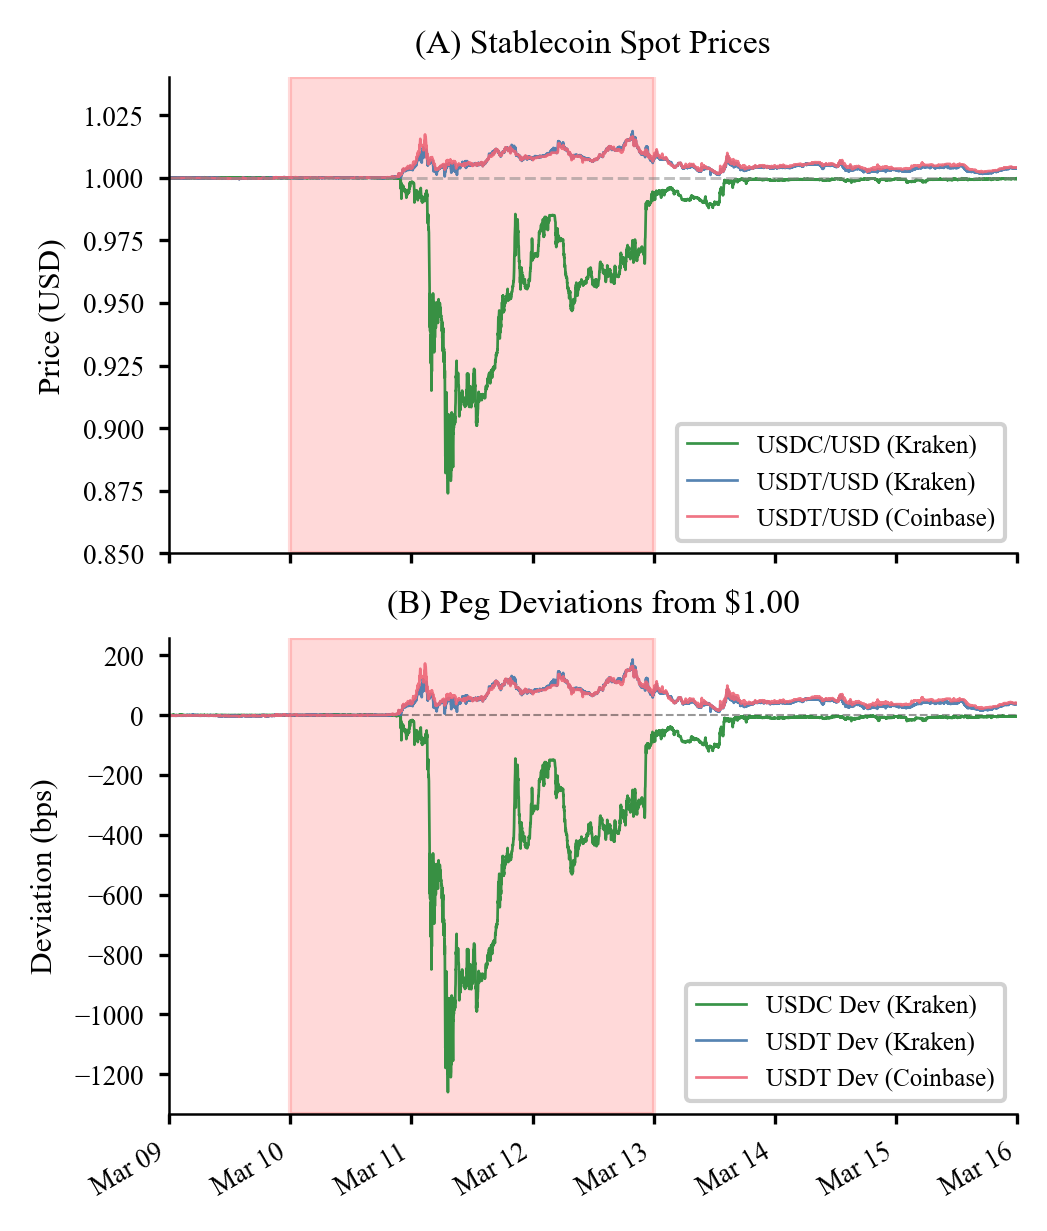
\includegraphics[width=\columnwidth]{figures_col/fig_stablecoin_peg.png}
    \caption{Stablecoin prices (A) and peg deviations (bps, B), March 2023. USDC falls to \$0.874; USDT trades at a premium. Shaded: SVB crisis (March 10--13, UTC).}
    \label{fig:peg}
\end{figure}

Our paper first decomposes this stablecoin driven fragmentation into a peg-deviation component and an adjusted residual. This reveals a $940\times$ half-life gap, which we statistically confirm via a moving-block bootstrap ($p{<}10^{-4}$), localizing the persistent dislocation strictly to the reserve-access layer. We then estimate a contagion intensity model to demonstrate that peg stress transmits to the adjusted basis well beyond the mechanical price channel. Specifically, we observe a transmission parameter $\hat\lambda$ that is significant ($p{<}0.001$) during the crisis but insignificant pre-SVB, reaffirming the two-layer linkage. Additionally, we observe pronounced asymmetry between USDC and USDT across tail risk, volatility, contagion direction, and cross-stablecoin correlation, an observation inconsistent with a symmetric common-shock explanation. Finally, we map these empirical findings to specific provisions of the GENIUS Act, providing a quantitative lens for evaluating the efficacy of structural stablecoin regulation.

The remainder of this paper is organized as follows: Section~\ref{sec:data} describes the data and methodology. Section~\ref{sec:results} presents the empirical results across five dimensions: dispersion decomposition, cross-exchange dispersion, market microstructure, price discovery, and arbitrage executability. Section~\ref{sec:regulation} interprets the findings through a regulatory policy lens, and Section~\ref{sec:conclusion} concludes.


% ======================================================================
\section{Data and Methodology}\label{sec:data}
% ======================================================================

\subsection{Data Sources and Processing}

To trace the propagation of peg stress, we create a high-frequency dataset of 1-minute OHLCV candles for Bitcoin across three distinct market microstructures. We select Binance for its dominance in global USDT volume, Coinbase as the primary U.S. fiat-to-crypto gateway, and Kraken for providing the most comprehensive suite of stablecoin-to-fiat pairs (including both USDC/USD and USDT/USD). This selection allows us to pair crypto-quoted assets with their exact venue-specific fiat conversion legs, ensuring that our calculated cross-currency bases are not contaminated by inter-exchange latency.

All raw series are synchronized to a unified 1-minute UTC grid (Table~\ref{tab:data_coverage}). While data coverage exceeds 97\% for the majority of series, pre-SVB Kraken BTC/USDC liquidity is notably thinner, with coverage dropping to 89.6\% and necessitating a 42\% forward-fill share. To preserve microstructural integrity, we restrict forward-filling to transient gaps of five minutes or less; larger discontinuities are left as missing values to prevent the injection of artificial autocorrelation into our mean-reversion estimates. Importantly, our core empirical findings, specifically the positive USDC crisis dispersion ($D_t > 0$) and the simultaneous USDT premium, remain directionally robust under strict no-forward-fill (no-FF) filtering.

\begin{table}[H]
\label{tab:data_coverage}
\footnotesize
\resizebox{\columnwidth}{!}{%
\begin{tabular}{lrrrrr}
\toprule
Pair & Coverage Overall (\%) & Coverage Pre-SVB (\%) & Coverage Crisis (\%) & Coverage Post-SVB (\%) & FF Share (\%) \\
\midrule
Kraken BTC/USD   & 99.98  & 100.00 & 100.00 & 99.95  & 0.18  \\
Kraken BTC/USDT  & 98.44  & 97.36  & 99.81  & 99.06  & 30.84 \\
Kraken BTC/USDC  & 94.05  & 89.62  & 99.79  & 96.57  & 42.07 \\
Kraken USDC/USD  & 97.80  & 96.03  & 99.35  & 99.06  & 28.57 \\
Kraken USDT/USD  & 99.98  & 100.00 & 100.00 & 99.95  & 0.91  \\
Coinbase BTC/USD & 99.10  & 97.90  & 100.00 & 100.00 & 0.06  \\
Coinbase BTC/USDT& 98.93  & 97.53  & 99.95  & 99.98  & 17.98 \\
Coinbase USDT/USD& 99.02  & 97.72  & 100.00 & 100.00 & 0.06  \\
Binance BTC/USDT & 100.00 & 100.00 & 100.00 & 100.00 & 0.00  \\
Binance BTC/USDC & 100.00 & 100.00 & 100.00 & 100.00 & 0.00  \\
\bottomrule
\end{tabular}%
}
\caption{1-minute data coverage and forward-fill exposure on the unified UTC grid. Coverage = non-missing share; FF share = carry-forward share (max 5 minutes).}
\end{table}

\subsection{Quantitative Framework}

To isolate stablecoin peg risk from broader breakdowns in market arbitrage, we first define the {unadjusted dispersion}, $D_{Q,t}$. For any stablecoin $Q\in\{\text{USDC}, \text{USDT}\}$, this captures the raw logarithmic price differential visible to a trader across quote currencies:
\begin{equation}
    D_{Q,t}=\left(\ln(P_{\text{BTC}/Q,t})-\ln(P_{\text{BTC/USD},t})\right)\times 10000.
\end{equation}

Because large de-pegs inflate $D_{Q,t}$, this metric conflates asset risk with numeraire risk. To extract the true microstructural arbitrage opportunity, we mark the stablecoin leg back to its realized USD value, yielding the {adjusted parity residual}, $B_{Q,t}$:
\begin{equation}
    \resizebox{0.92\columnwidth}{!}{$\displaystyle
    B_{Q,t} = \left(\ln(P_{\text{BTC}/Q,t}\times P_{Q/\text{USD},t})-\ln(P_{\text{BTC/USD},t})\right)\times 10000.
    $}
\end{equation}

By satisfying $B_{Q,t}=D_{Q,t}+10000\cdot\ln(P_{Q/\text{USD},t})$, this decomposition localizes the dislocation: an immense $D_t$ coupled with a compressed $B_t$ proves the breakdown resides almost entirely in the peg layer. Both metrics are computed intra-exchange to eliminate cross-venue latency. 

Theoretical gaps, however, do not immediately translate to executable arbitrage. A 320 bps dispersion appears massive, but standard triangular arbitrage incurs significant taker fees and market impact. To conservatively proxy execution costs without historical order-book depth, we utilize the intra-minute range:
\begin{equation}
    \resizebox{0.92\columnwidth}{!}{$\displaystyle
    \text{Intra-min Range (bps)} = \left( \frac{\text{High}_t - \text{Low}_t}{\text{Close}_t} \right)\times 10000.
    $}
\end{equation}
Applying this friction strictly bounds the profitability of $B_t$, demonstrating how seemingly massive structural dislocations compress under realistic trading conditions.

Once $B_t$ is isolated and friction-bounded, we quantify its temporal decay. We model $B_t$ as a mean-reverting Ornstein--Uhlenbeck (OU) process, estimating its discrete-time AR(1) analog ($X_t = c + \rho X_{t-1} + \varepsilon_t$) to extract the half-life of the dislocation:
\begin{equation}
    \tau_{1/2} = \frac{\ln(2)\,\Delta t}{-\ln(\rho)}, \quad 0<\rho<1.
\end{equation}
To validate the resulting gap between the peg half-life (${\approx}572$ min) and the basis half-life (${\approx}0.6$ min), standard parametric intervals are insufficient, as the peg's $\hat\rho \approx 0.999$ borders the unit-root boundary, leading to instability. We instead deploy a 60-minute moving-block bootstrap. This preserves local dependency structures, giving us a robust empirical distribution and a precise $p$-value for the efficiency gap.

While this separates $B_t$ and $D_t$, we want to observe if banking-layer stress actively infects crypto-native liquidity. To formalize this, we extend the mean-reversion equation into a contagion intensity model by introducing the lagged peg deviation $S_{t-1}$ (in bps) as a forcing variable:
\begin{equation}\label{eq:contagion}
    \Delta B_t = a + \beta\, B_{t-1} + \lambda\, S_{t-1} + \varepsilon_t.
\end{equation}
A statistically significant transmission parameter ($\hat\lambda \neq 0$) proves that peg stress actively leaks into the arbitrage basis via microstructure channels like liquidity withdrawal. We estimate this via OLS with Newey--West HAC standard errors (60 lags) to account for high-frequency serial correlation, while the lagged structure inherently prevents simultaneity bias.

As these layers decouple, we map where true price discovery anchors. If BTC cross-currency pairs share a stochastic trend, their deviations are transitory, making a Vector Error Correction Model (VECM) the optimal specification. Following Johansen trace tests, we estimate the structural adjustment:
\begin{equation}
    \Delta \mathbf{p}_t = \alpha \beta^\top \mathbf{p}_{t-1} + \sum_{i=1}^{k_{\Delta}} \Gamma_i \Delta \mathbf{p}_{t-i} + \mathbf{u}_t.
\end{equation}
The market exhibiting the smaller adjustment coefficient $|\alpha|$ is the relative leader. Using Hasbrouck (1995) Information Shares, which explicitly test the economic intuition that deeper fiat markets dominate price formation during systemic stablecoin stress we establish this leadership .

Crucially, we execute this entire sequence independently across pre-SVB, crisis, and post-SVB windows. Chow tests overwhelmingly reject parameter stability at the March 10 break ($F > 2000$), dictating that a pooled model would impose an artificial functional form. Regime-specific estimation ensures our framework organically adapts to the shifting structural realities of the crisis.

% ======================================================================
\section{Empirical Results}\label{sec:results}
% ======================================================================

\subsection{Dispersion, adjusted residual, and mean reversion}

To quantify the magnitude of the SVB dislocation, we first evaluate the baseline market conditions. Before the crisis, both unadjusted dispersion ($D_t$) and the adjusted parity residual ($B_t$) were near zero across all channels. However, during the crisis window, the market fractured. Table~\ref{tab:dispersion_vs_adjusted} reveals that USDC dispersion surged to a mean of $+320$ bps ($\sigma{=}323$), yet the adjusted residual remained remarkably compressed at just $+5.3$ bps ($\sigma{=}21$). Conversely, USDT moved in the opposite direction, registering $D_t{=}{-}57$ bps and $B_t{=}{+}0.7$ bps. 

\begin{table}[H]
\label{tab:dispersion_vs_adjusted}
\footnotesize
\resizebox{\columnwidth}{!}{%
\begin{tabular}{llrrrr}
\toprule
Regime & Series & Mean (bps) & Std (bps) & Mean Abs (bps) & N \\
\midrule
Pre-SVB  & USDC $D_t$ (Unadj.) &    0.12 &   4.95 &   3.49 & 11615 \\
Pre-SVB  & USDC $B_t$ (Adj.)   &   -0.32 &   5.00 &   3.53 & 11197 \\
Pre-SVB  & USDT $D_t$ (Unadj.) &   -0.54 &   4.49 &   3.17 & 12618 \\
Pre-SVB  & USDT $B_t$ (Adj.)   &   -0.60 &   4.33 &   3.02 & 12618 \\
Crisis   & USDC $D_t$ (Unadj.) &  319.97 & 322.87 & 321.17 &  4311 \\
Crisis   & USDC $B_t$ (Adj.)   &    5.27 &  21.21 &  13.37 &  4283 \\
Crisis   & USDT $D_t$ (Unadj.) &  -57.18 &  45.10 &  58.57 &  4312 \\
Crisis   & USDT $B_t$ (Adj.)   &    0.68 &   6.57 &   4.94 &  4312 \\
Post-SVB & USDC $D_t$ (Unadj.) &   11.22 &  21.95 &  14.27 & 12514 \\
Post-SVB & USDC $B_t$ (Adj.)   &    0.45 &   9.06 &   6.68 & 12419 \\
Post-SVB & USDT $D_t$ (Unadj.) &  -30.26 &  13.29 &  30.28 & 12837 \\
Post-SVB & USDT $B_t$ (Adj.)   &   -1.23 &   6.47 &   4.92 & 12837 \\
\bottomrule
\end{tabular}%
}
\caption{Kraken regime statistics for unadjusted dispersion ($D_t$) and adjusted residual ($B_t$), in bps.}
\end{table}

\newpage

\begin{figure}[H]
    \centering
    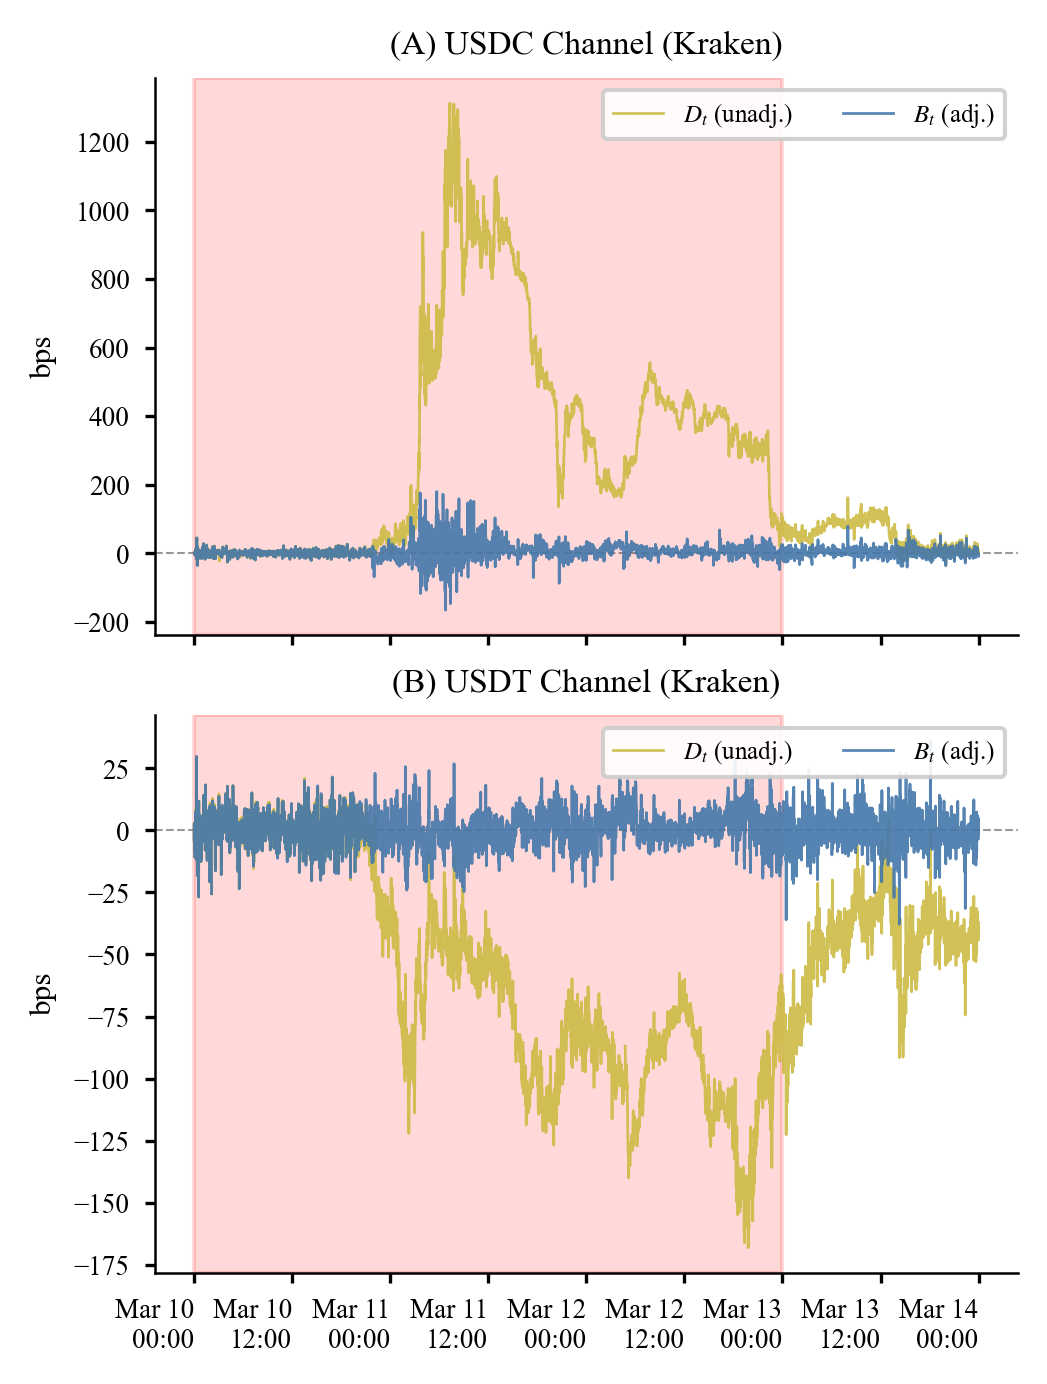
\includegraphics[width=\columnwidth]{figures_col/fig_dispersion_vs_adjusted_kraken.png}
\caption{Kraken crisis decomposition. USDC unadjusted dispersion spikes past $+1200$ while the adjusted residual remains bounded within $\pm150$.}
    \label{fig:decomp}
\end{figure}

\begin{figure}[H]
    \centering
    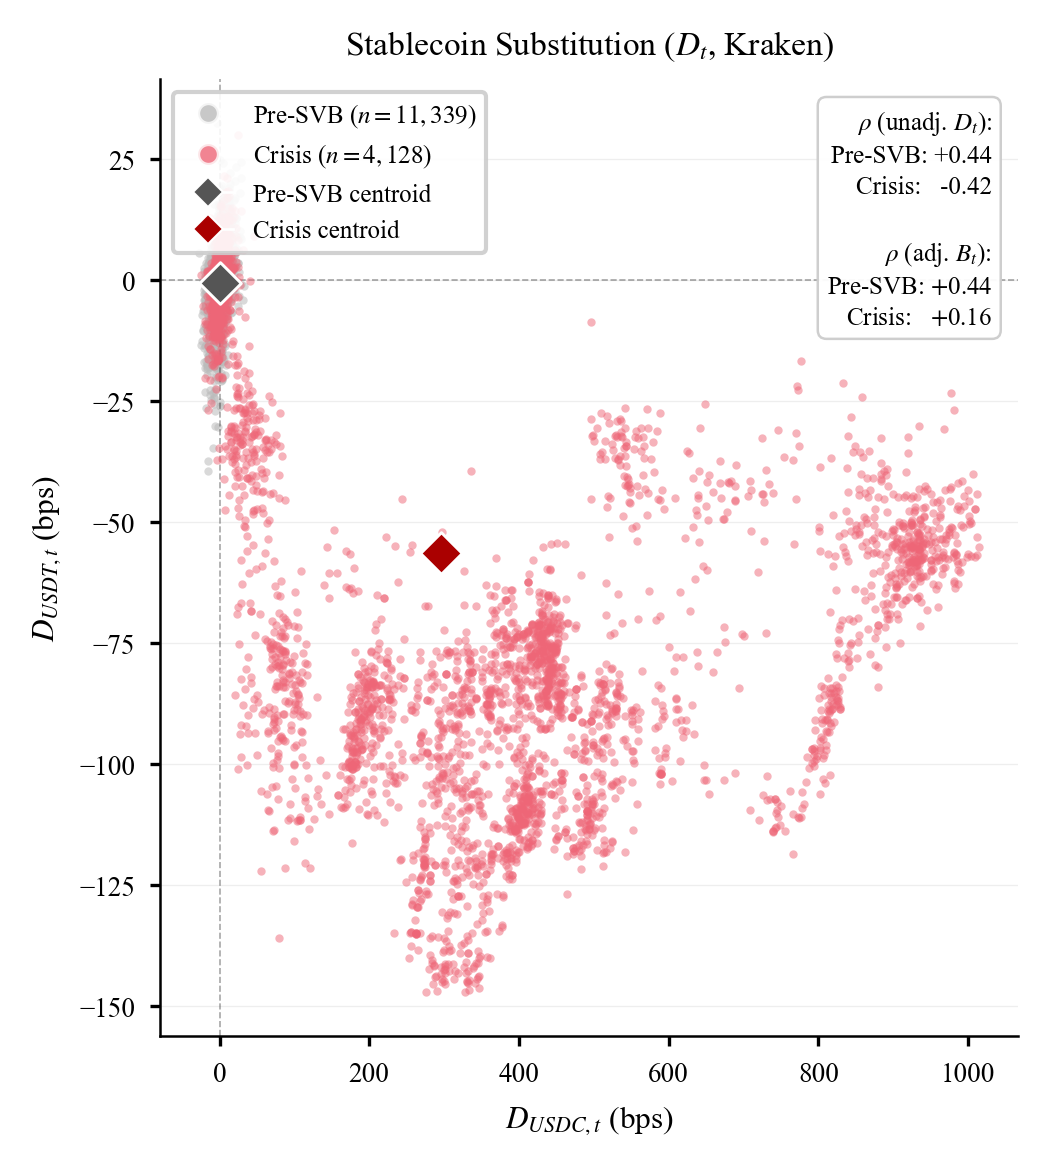
\includegraphics[width=\columnwidth]{figures_col/fig_stablecoin_substitution_scatter.png}
\caption{Stablecoin substitution dynamics. Crisis observations migrate to the lower-right, flipping unadjusted correlation ($+0.44\to-0.42$) and dropping $B_t$ correlation to $0.16$.}
    \label{fig:substitution}
\end{figure}

To ensure these observed shifts are not microstructural artifacts, we compute HAC/Newey--West intervals (60-lag cap) \cite{neweywest1987}, which confirm directional robustness. The USDC crisis $D_t$ 95\% CI spans $[245.7,\,394.3]$ bps, while the $B_t$ CI remains tightly bounded at $[3.6,\,7.0]$ bps. The USDT premiums are confirmed positive on both Kraken ($[47.4,\,68.8]$) and Coinbase ($[49.1,\,70.3]$), and the cross-exchange Coinbase--Kraken BTC/USD fiat basis remains significantly elevated ($[1.7,\,2.6]$ bps).

\begin{figure}[H]
    \centering
    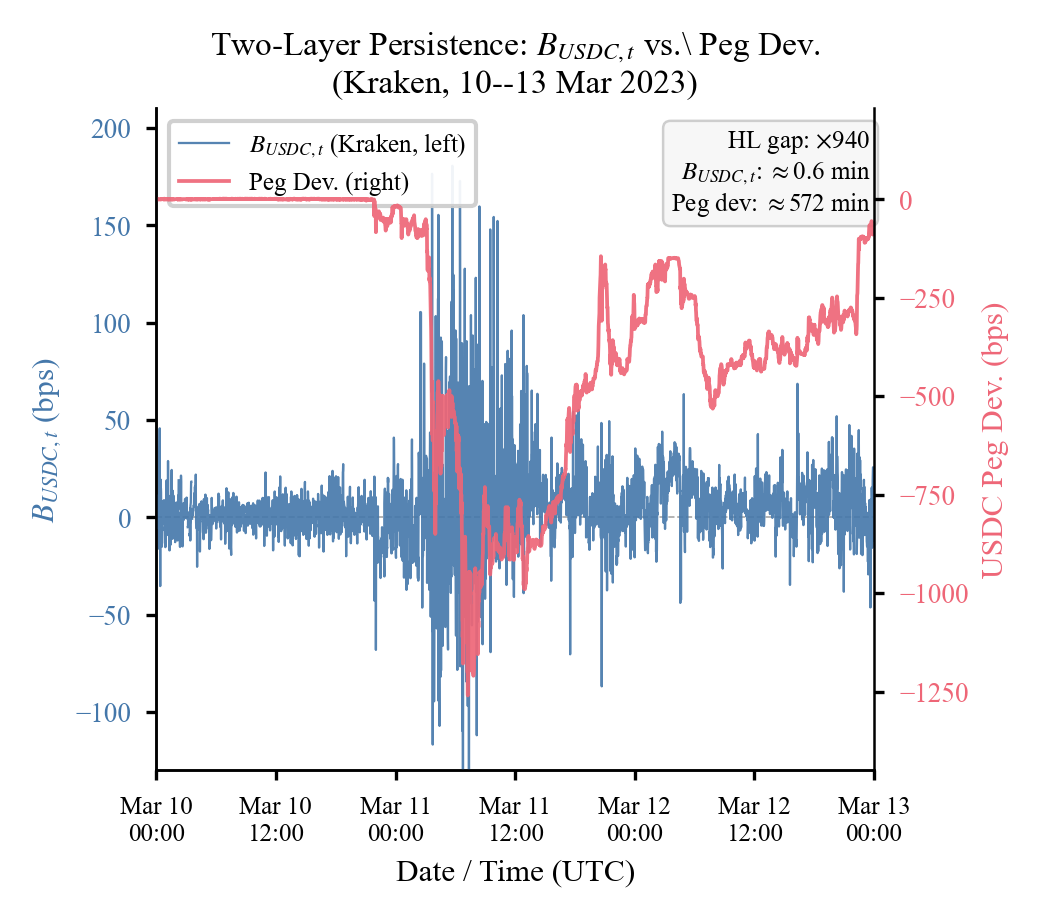
\includegraphics[width=\columnwidth]{figures_col/fig_two_layer_persistence.png}
    \caption{Two-layer persistence (March 10--13): $B_{\text{USDC},t}$ mean-reverts in ${\approx}0.6$ min, while the USDC peg deviation persists for ${\approx}572$ min. The ${\sim}940\times$ gap localizes persistent dislocation to the peg layer.}
    \label{fig:twolayer}
\end{figure}

Having established the magnitude of the dislocation, we evaluate its temporal persistence. ADF tests overwhelmingly reject a unit root for all $B_t$ channels ($p<0.001$). Our Ornstein-Uhlenbeck (OU) estimation uncovers a {two-layer dynamic} (Figure~\ref{fig:twolayer}). We see that the adjusted basis $B_t$ mean-reverts in just ${\approx}0.6$ min during the crisis ($\hat\rho{=}0.320$), whereas the underlying USDC peg deviation persists with a half-life of ${\approx}572$ min ($\hat\rho{=}0.999$, ADF $p{=}0.44$). USDT peg deviations display similar persistence ($496$--$542$ min). 

Because the resulting point-estimate ratio $R{=}\tau_{1/2}^{\text{peg}}/\tau_{1/2}^{B}{\approx}940$ could theoretically be an artifact of estimation noise near the unit-root boundary, we validate it using a moving-block bootstrap (5{,}000 replications; block length 60 minutes). This give us an $R_{\text{median}}{=}567$ with a 95\% CI of $[216,\,1{,}898]$ and $p{<}10^{-4}$ for the null $H_0{:}\;R{\le}1$. This statistically persistence gap proves that while cross-market crypto arbitrage corrects almost instantly, the true dislocation remains trapped in the fiat-reserve layer. This high-frequency efficiency is highly robust, as Figure~\ref{fig:halflife_robust} confirms that across 1m/5m sampling and no-forward-fill filters, the USDC crisis half-life consistently remains between $0.54$ and $1.10$ min, while USDT exhibits slightly longer persistence ($0.92$--$3.06$ min).

% Full-width figure (dot-plot across regimes/specs)
\begin{figure}[H]
    \centering
    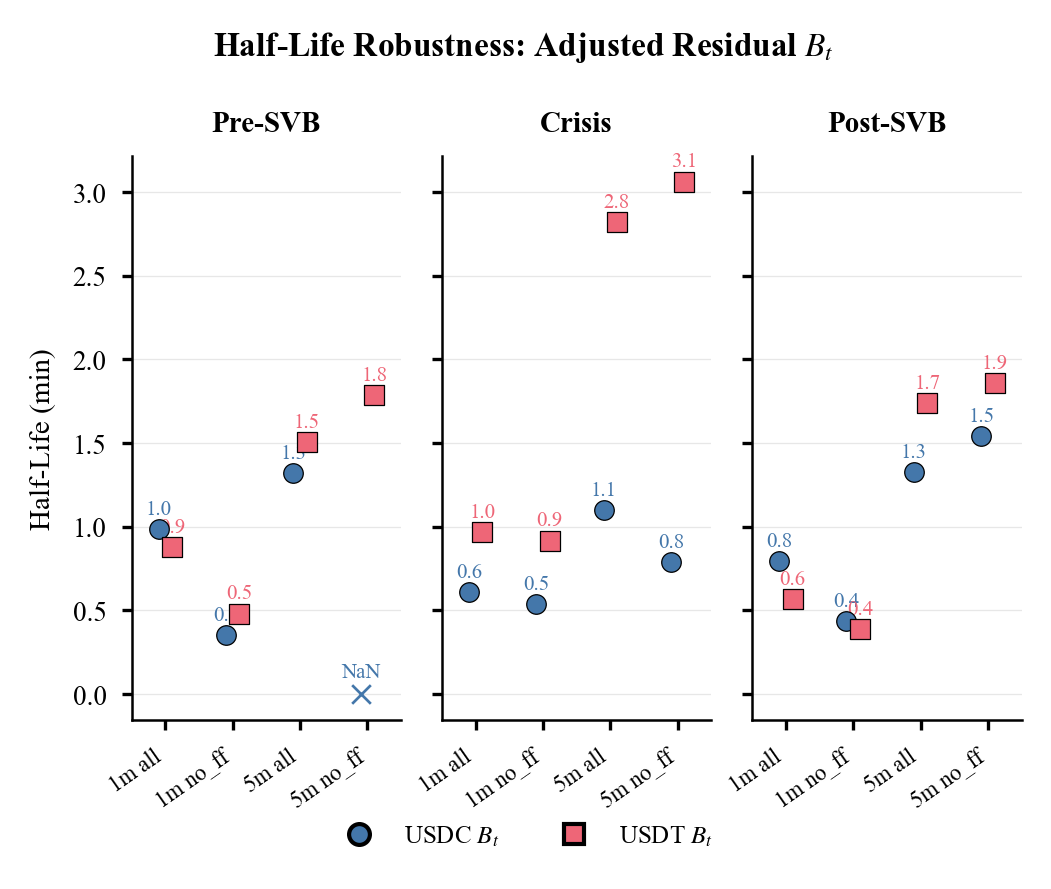
\includegraphics[width=\columnwidth]{figures_col/fig_half_life_robustness.png}
    \caption{Adjusted-residual $B_t$ half-life robustness by regime/specification (1m/5m $\times$ all/no-FF). USDC crisis half-life stays below 1.1 min; USDT reaches 3.1 min (5m no-FF).}
    \label{fig:halflife_robust}
\end{figure}



\paragraph{Contagion intensity.}
While the two-layer dynamic isolates the persistence of the shock, we must determine if the layers interact economically beyond their decomposition. Estimating the coupled contagion model~(\ref{eq:contagion}), we discover that the transmission parameter $\hat\lambda$ is indistinguishable from zero pre-SVB ($-0.002$, $p{=}0.98$), but becomes significant during the crisis ($-0.009$, $p{<}0.001$) and remains elevated post-SVB ($-0.019$, $p{=}0.006$), as detailed in Table~\ref{tab:contagion}. 

\begin{table}[H]
\label{tab:contagion}
\footnotesize
\centering
\resizebox{\columnwidth}{!}{%
\begin{tabular}{llrrrrrr}
\toprule
Channel & Regime & $\hat\lambda$ & SE & $t$-stat & $p$-value & $R^2$ & $N$ \\
\midrule
USDC & Pre-SVB  & $-$0.002 & 0.091 & $-$0.02 & 0.985 & 0.253 & 11{,}196 \\
USDC & Crisis   & $-$0.009 & 0.002 & $-$4.77 & ${<}0.001$ & 0.351 & 4{,}282 \\
USDC & Post-SVB & $-$0.019 & 0.007 & $-$2.73 & 0.006 & 0.293 & 12{,}418 \\
\midrule
USDT & Pre-SVB  & $-$0.076 & 0.032 & $-$2.38 & 0.017 & 0.273 & 12{,}617 \\
USDT & Crisis   & $+$0.019 & 0.004 & $+$5.23 & ${<}0.001$ & 0.272 & 4{,}311 \\
USDT & Post-SVB & $+$0.023 & 0.008 & $+$2.80 & 0.005 & 0.354 & 12{,}836 \\
\bottomrule
\end{tabular}%
}
\caption{Contagion intensity $\hat\lambda$ from Eq.~(\ref{eq:contagion}): regime-specific OLS with Newey--West HAC (60 lags). $S_t$ is the peg deviation (bps; negative = discount).}
\end{table}

Because $S_t{<}0$ represents a peg discount, the negative $\hat\lambda$ implies that a deeper USDC discount at $t{-}1$ pushes the arbitrage basis $B_t$ upward at $t$. This is consistent with liquidity withdrawal from the USDC order book, which creates a positive residual basis even after marking to USD. USDT displays the mirror pattern, as $\hat\lambda{=}{+}0.019$ during the crisis ($p{<}0.001$). Here, a USDT premium at $t{-}1$ pulls $B_t$ upward, confirming that safe-haven demand actively spills into the adjusted residual. For both stablecoins, these sign patterns confirm that peg stress does not merely drive $D_t$, but actively infects $B_t$ through market microstructure channels.

\begin{figure}[H]
    \centering
    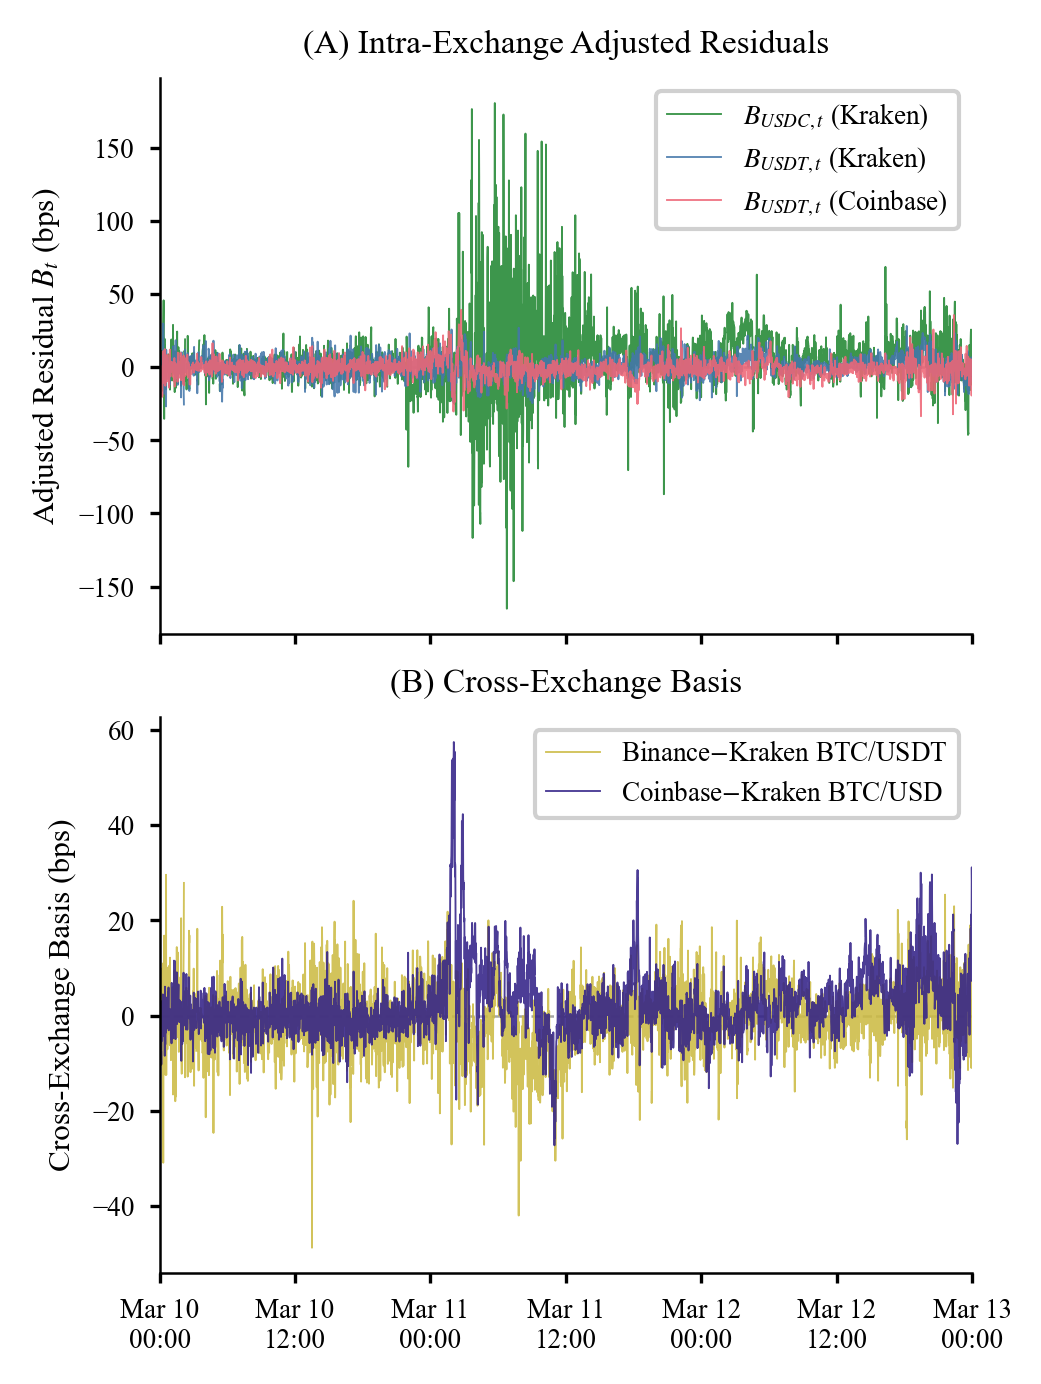
\includegraphics[width=\columnwidth]{figures_col/fig_svb_crisis_zoom.png}
    \caption{Crisis zoom (March 10--13).}
    \label{fig:crisiszoom}
\end{figure}

These transmission dynamics are highly robust, holding significance for USDC under no-forward-fill sampling ($-0.009$, $p{<}0.001$, $N{=}3{,}001$) and at the 5-minute frequency ($-0.012$, $p{<}0.001$, $N{=}861$). Furthermore, the USDT sign flip from pre-SVB ($\hat\lambda{<}0$) to crisis ($\hat\lambda{>}0$) coincides perfectly with the systemic shift toward safe-haven dynamics. 

To observe this contagion at the micro-level, Figure~\ref{fig:crisiszoom} provides a granular minute-by-minute view of the peak crisis window. Panel~A reveals extreme volatility in the USDC adjusted residual ($B_{\text{USDC},t}$), which violently spikes past $\pm150$ bps, while USDT channels remain strictly bounded within $\pm30$ bps. Simultaneously, Panel~B demonstrates that the cross-exchange basis widens in tandem, with the Coinbase--Kraken BTC/USD differential surging to $+60$ bps. Together, these dynamics provide a clear visual testament to how localized stablecoin dislocations rapidly propagate as systemic stress across multiple venues.

\subsection{Cross-exchange price dispersion}

\begin{figure}[H]
    \centering
    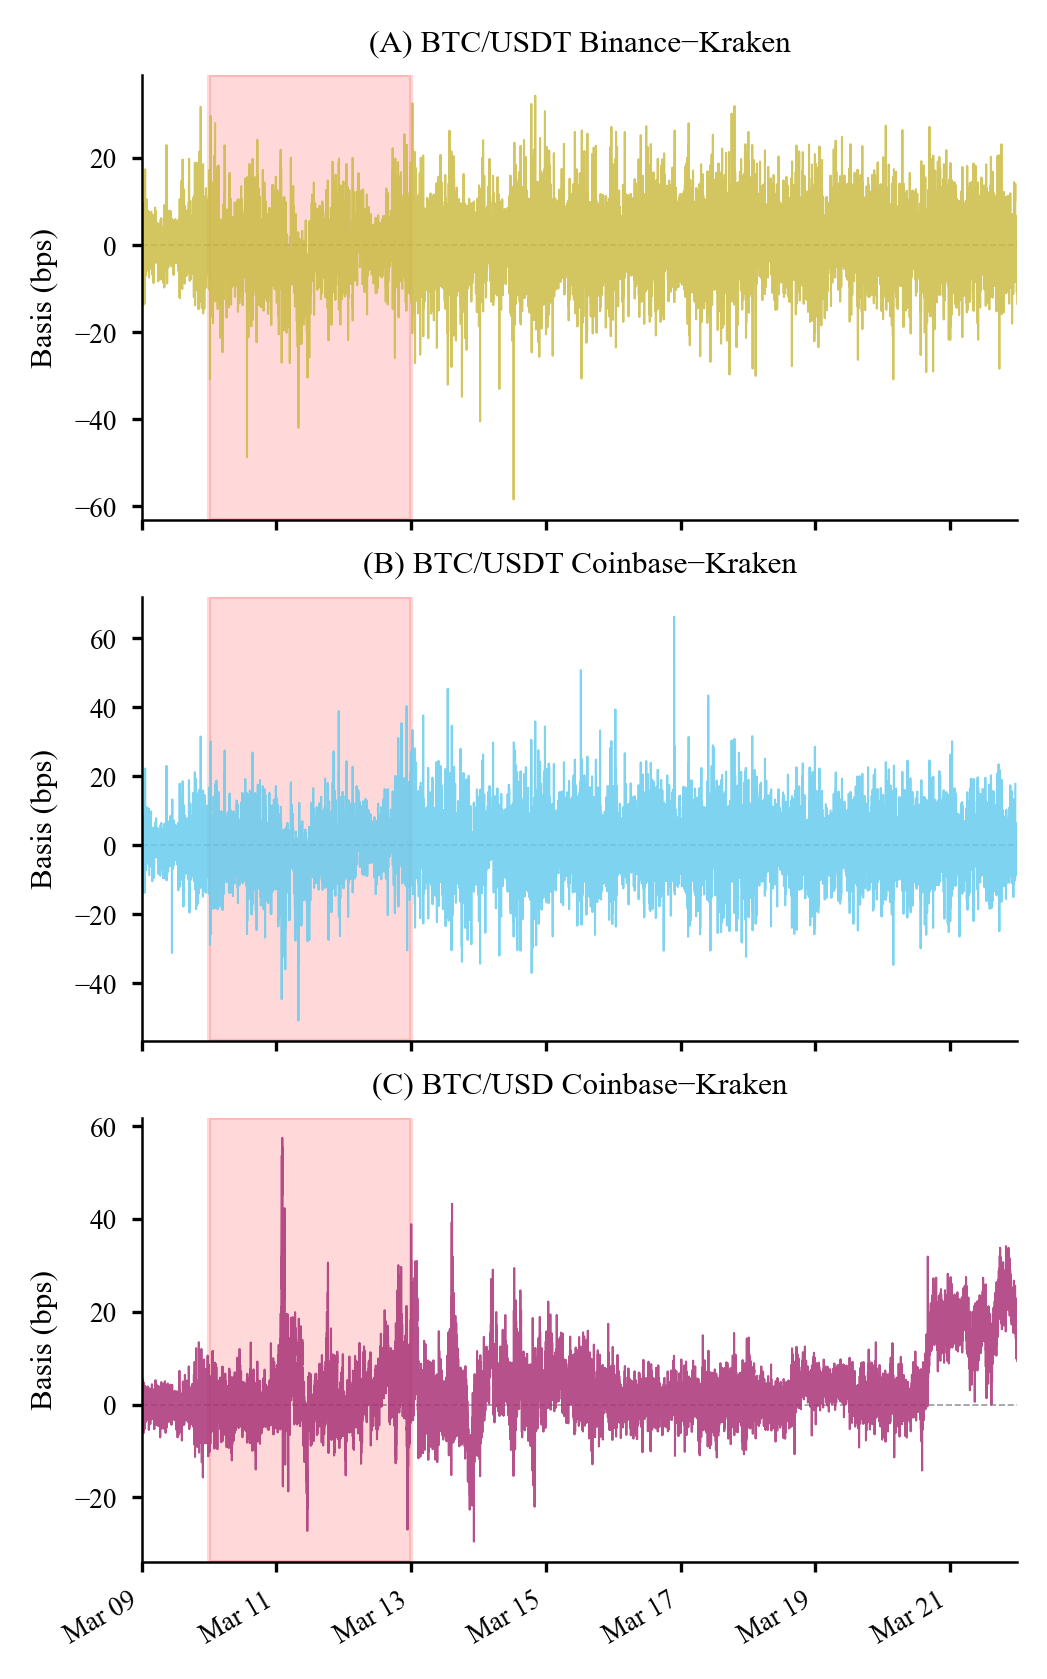
\includegraphics[width=\columnwidth]{figures_col/fig_cross_exchange_basis.png}
    \vspace{-15pt}     
    \caption{Cross-exchange basis during crisis}
    \label{fig:xbasis}
    \vspace{-10pt}
\end{figure}

Having established that intra-exchange fragmentation is dominated by USDC peg risk, we investigate whether this dislocation propagates {across} exchanges. Figure~\ref{fig:xbasis} maps these log-price differentials (in bps) across three distinct channels: BTC/USDT for Binance--Kraken (Panel A) and Coinbase--Kraken (Panel B), alongside the fiat BTC/USD pair for Coinbase--Kraken (Panel C). Because USDT cross-exchange dispersion is denominated in the USDT numeraire, any USD-based arbitrage mechanically requires an additional USDT/USD conversion leg. 

Under baseline conditions, the Binance--Kraken BTC/USDT differential remains near zero ($+0.007$ bps full-sample). During the crisis, however, cross-exchange differentials widen uniformly alongside the intra-exchange deviations documented above (Table~\ref{tab:arb}), confirming that the shock was a broad systemic event rather than a single-venue disruption. Most notably, the Coinbase--Kraken fiat channel (Panel C) exhibits a persistent $+2.18$ bps premium that remains elevated even post-crisis. This suggests the U.S. fiat gateway premium did not fully normalize, reflecting underlying structural microstructure differences that the SVB shock permanently amplified.

\subsection{Market microstructure dynamics}\label{sec:liq_vol}

\begin{figure}[H]
    \centering
    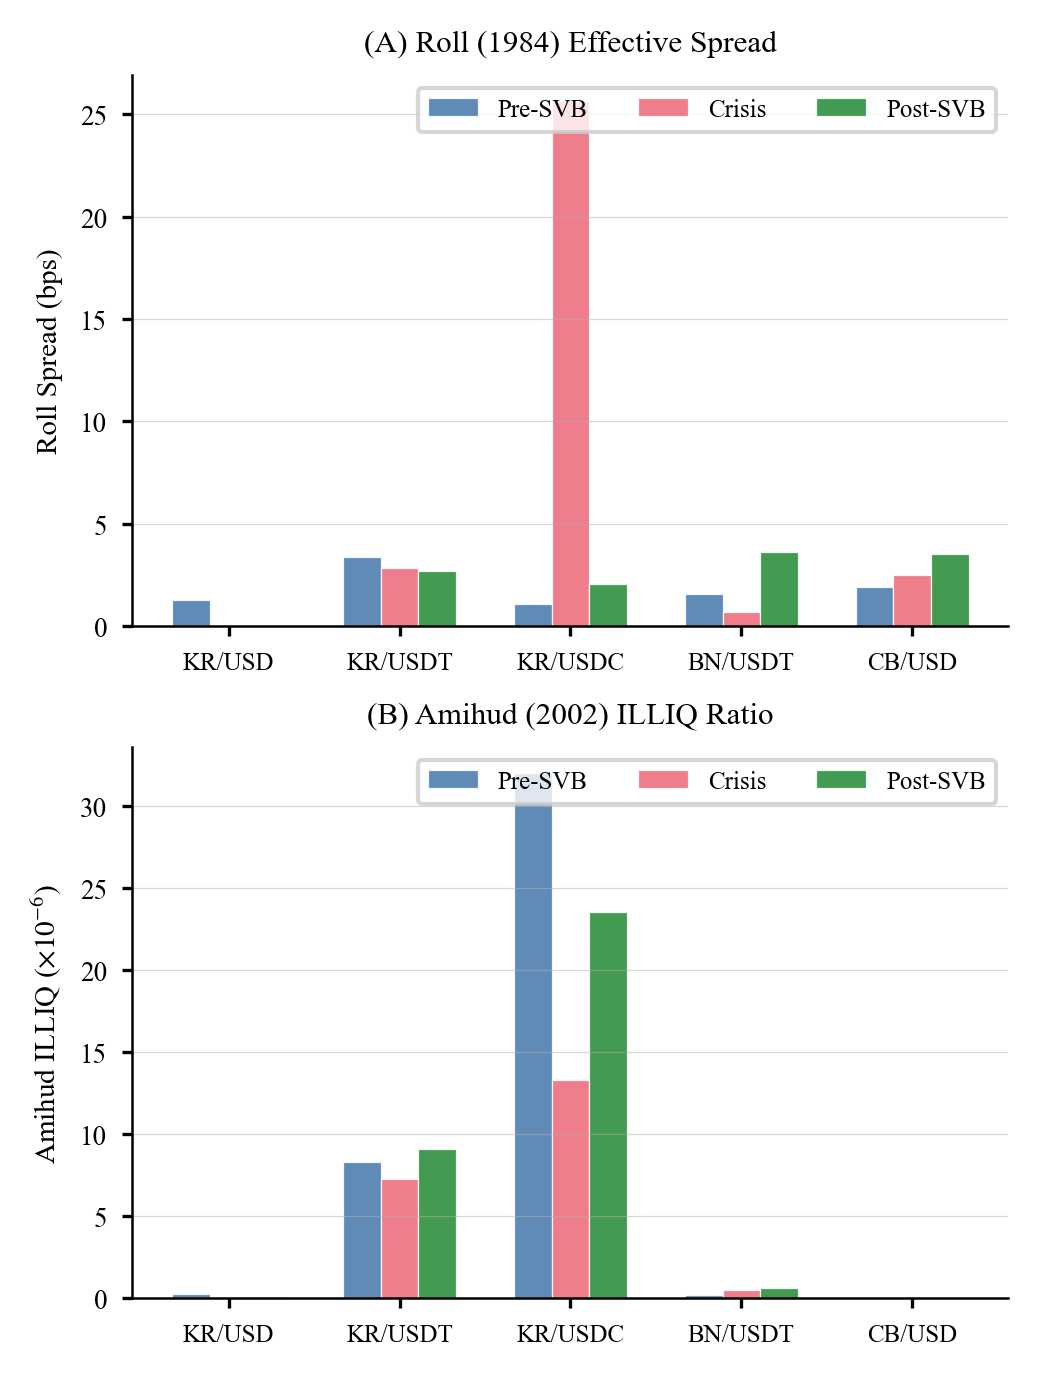
\includegraphics[width=\columnwidth]{figures_col/fig_liquidity_roll_amihud.png}
    \vspace{-15pt}     
    \caption{Roll effective \& Amihud by pair/regime.}
    \label{fig:liq}
    \vspace{-10pt}
\end{figure}

The cross-exchange widening documented above raises the question of whether liquidity conditions differ across channels. To quantify this microstructural friction, we utilize the Roll (1984) effective spread \cite{roll1984} and Amihud (2002) ILLIQ ratio \cite{amihud2002}. As detailed in Table~\ref{tab:liquidity_spread} and Figure~\ref{fig:liq} (Panels A and B), the Kraken BTC/USDC Roll spread experiences a $23\times$ blowout during the crisis (jumping from $1.10$ to $25.64$ bps), whereas BTC/USDT remains stable near $3$ bps. Because the Roll measure is undefined when serial covariance is non-negative, thin-pair means are strictly indicative. Nevertheless, the Amihud ratio confirms that Coinbase BTC/USD serves as the deepest venue while Kraken BTC/USDC is the thinnest. Notably, these two metrics actively diverge during stress. We observe that Roll spreads widen as quoting friction increases, while the Amihud ratio declines due to surging aggregate volume.

\begin{table}[H]
\label{tab:liquidity_spread}
\footnotesize
\resizebox{\columnwidth}{!}{%
\begin{tabular}{lrrrrrrrrr}
\toprule
Pair & Roll\textsubscript{Pre} & Roll\textsubscript{Crisis} & Roll\textsubscript{Post} & $N$\textsubscript{Pre} & $N$\textsubscript{Crisis} & $N$\textsubscript{Post} & ILLIQ\textsubscript{Pre} & ILLIQ\textsubscript{Crisis} & ILLIQ\textsubscript{Post} \\
\midrule
Kraken BTC/USD  & 1.260 & ---    & ---   & 4 & 0 & 0 & 0.232  & 0.050  & 0.068  \\
Kraken BTC/USDT & 3.390 & 2.850  & 2.670 & 1 & 1 & 1 & 8.299  & 7.266  & 9.074  \\
Kraken BTC/USDC & 1.100 & 25.640 & 2.070 & 2 & 2 & 2 & 31.970 & 13.282 & 23.530 \\
Binance BTC/USDT& 1.560 & 0.670  & 3.630 & 6 & 1 & 5 & 0.163  & 0.461  & 0.591  \\
Coinbase BTC/USD& 1.880 & 2.490  & 3.490 & 5 & 1 & 1 & 0.005  & 0.003  & 0.003  \\
\bottomrule
\end{tabular}%
}
\caption{Roll effective spread (bps) and Amihud illiquidity ($\times10^{-6}$) by pair/regime.}
\end{table}

Daily dollar-volume depth proxies (Table~\ref{tab:depth_proxy}) sharpen this picture: Coinbase BTC/USD is the deepest channel (\$239M pre-SVB, rising to \$664M post-SVB), while Kraken BTC/USDC is $26\times$ thinner in crisis (\$15.7M vs.\ \$407M). The depth gap constrains the scale at which arbitrageurs can trade the USDC dislocation, consistent with the limited post-friction profitability documented in Section~\ref{sec:arb}.

\begin{table}[H]
\label{tab:depth_proxy}
\footnotesize
\resizebox{\columnwidth}{!}{%
\begin{tabular}{lrrr}
\toprule
Pair & Pre-SVB & Crisis & Post-SVB \\
\midrule
Kraken BTC/USD   & 59.50  & 160.36 & 203.77 \\
Kraken BTC/USDT  &  5.55  &  13.84 &  17.37 \\
Kraken BTC/USDC  &  2.56  &  15.65 &   5.52 \\
Binance BTC/USDT & 52.44  &  73.92 &  71.46 \\
Coinbase BTC/USD & 239.07 & 407.27 & 664.46 \\
\bottomrule
\end{tabular}%
}
\caption{Daily traded dollar volume by pair/regime (median, \$MM/day)}
\end{table}

HAC regressions (Newey--West, 60 lags) of $B_t$ on a crisis dummy, realized volatility, and range proxy (Table~\ref{tab:regression_hac}) show a significant USDC crisis coefficient ($+4.30$ bps, $p<0.001$) \cite{neweywest1987}. However, the explanatory power is modest ($R^2=0.041$), so we interpret these as partial associations.

\begin{table}[H]
\label{tab:regression_hac}
\footnotesize
\centering
\resizebox{\columnwidth}{!}{%
\begin{tabular}{lcccc}
\toprule
 & \multicolumn{2}{c}{USDC Channel} & \multicolumn{2}{c}{USDT Channel} \\
\cmidrule(lr){2-3} \cmidrule(lr){4-5}
 & Coef. & $p$-value & Coef. & $p$-value \\
\midrule
Constant          & $-0.079$ & 0.833   & $-0.656$ & $<0.001$ \\
Crisis            & $+4.295$ & $<0.001$& $+1.655$ & $<0.001$ \\
RealizedVol (60m) & $+0.004$ & 0.928   & $-0.029$ & 0.179    \\
Range Proxy       & $+0.048$ & 0.005   & $-0.013$ & 0.082    \\
\midrule
$R^2$             & \multicolumn{2}{c}{0.041}  & \multicolumn{2}{c}{0.012}  \\
$N$               & \multicolumn{2}{c}{26,489} & \multicolumn{2}{c}{26,489} \\
\bottomrule
\multicolumn{5}{l}{\footnotesize OLS with HAC standard errors (Newey--West, 60 lags). Dependent variable: $B_t$ (bps).}
\end{tabular}%
}
\caption{HAC regressions of Kraken adjusted residual $B_t$}
\end{table}

% Full-width figureyszx
\begin{figure}
    \centering
    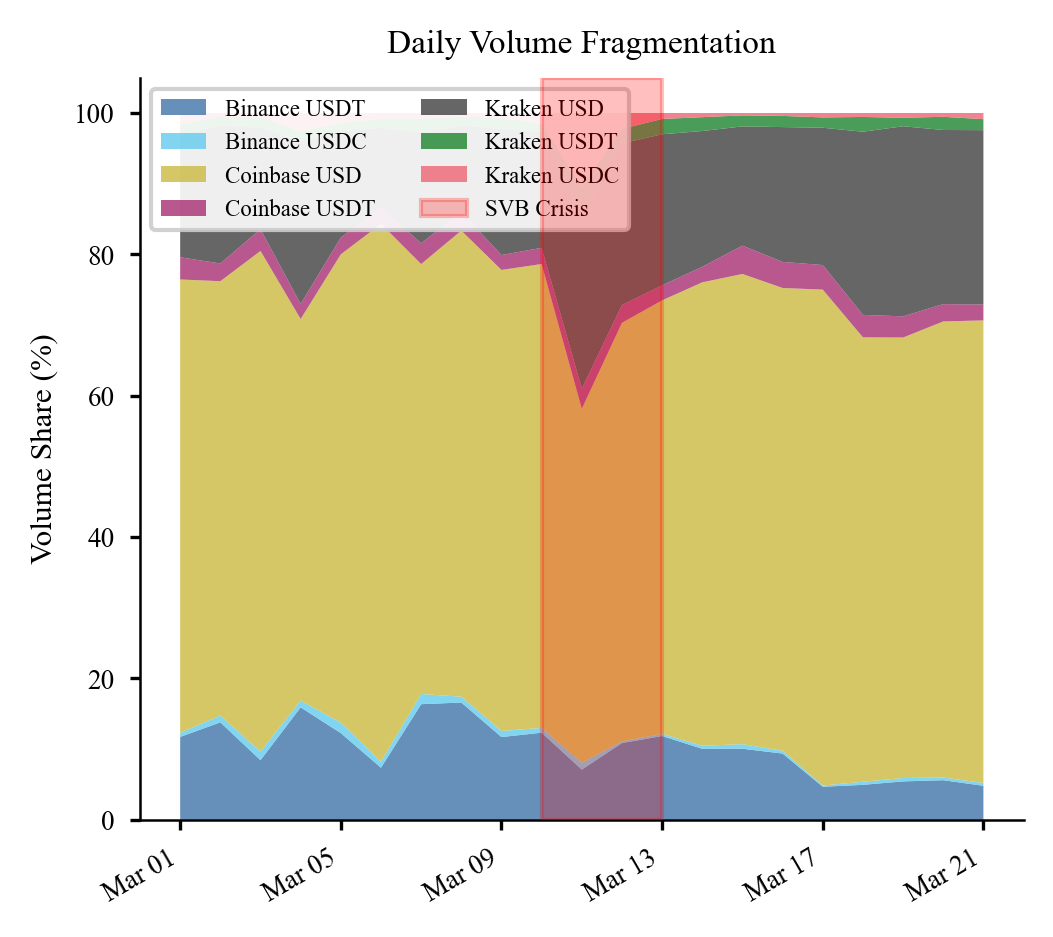
\includegraphics[width=\columnwidth]{figures_col/fig_volume_share.png}
    \caption{Daily volume shares across pairs. USDC share spikes during the crisis (Kraken BTC/USDC surge) and rotates back to USD post-crisis.}
    \label{fig:volshare}
\end{figure}

Figure~\ref{fig:volshare} shows daily volume fragmentation: USDC share doubles during crisis (2.1\% to 4.3\%) as activity concentrates in Kraken BTC/USDC, while post-crisis USD dominance returns (86.9\%).

Realized volatility (Figure~\ref{fig:realvol}) reveals strong asymmetry: Kraken BTC/USDC peaks at ${\approx}650$ bps/hr on March 11, roughly $2.1\times$ the crisis-average for BTC/USD and BTC/USDT, which is consistent with compounding asset risk and numeraire risk.

The distributional impact is very significant (Figure~\ref{fig:tailblowout}). We see crisis USDC $B_t$ develops tails beyond $\pm100$ bps versus $\pm10$ bps pre-SVB. For risk management, stablecoin positions carry latent peg-break tail risk that calm-calibrated VaR models consistently understate.

% Full-width figure
\begin{figure}[H]
    \centering
    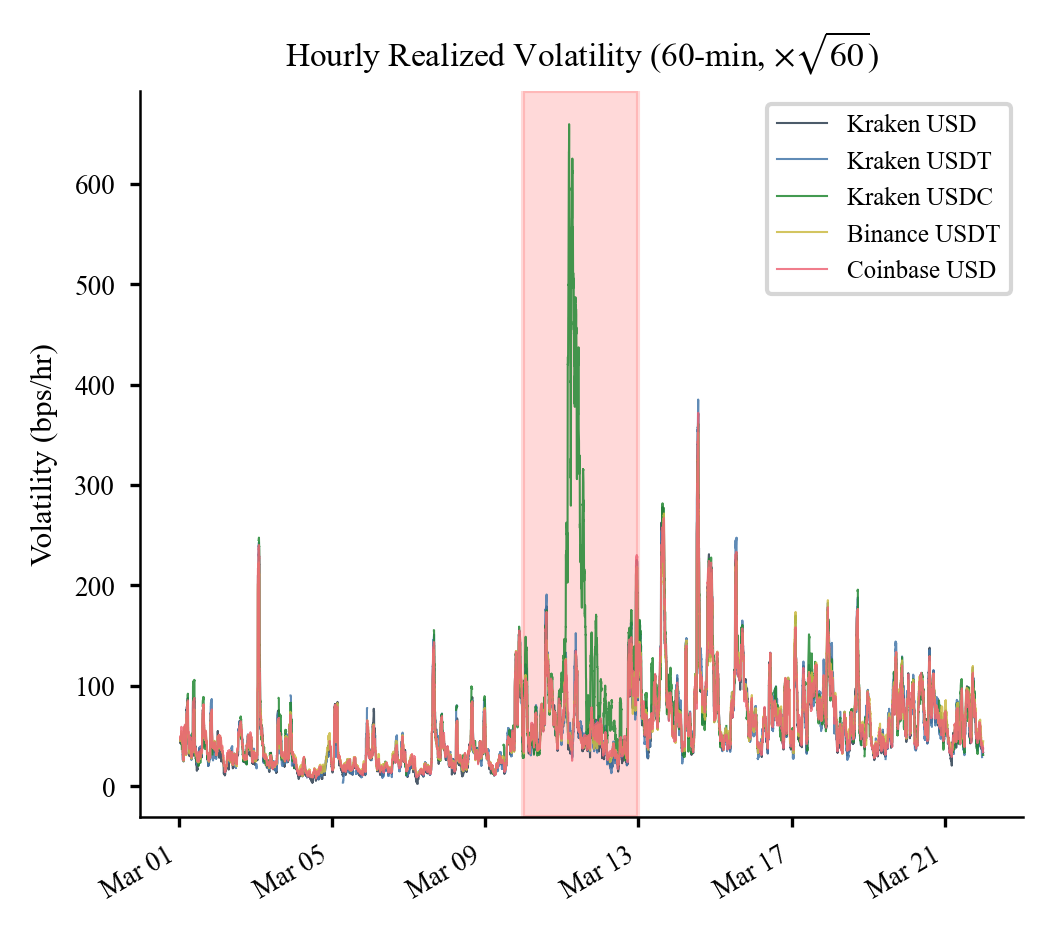
\includegraphics[width=\columnwidth]{figures_col/fig_realized_volatility.png}
    \caption{Hourly realized volatility (60-min rolling $\sigma$, $\times\sqrt{60}$) by pair. Kraken BTC/USDC peaks near ${\approx}650$ bps/hr in crisis, about $2.1\times$ the USD and USDT channels.}
    \label{fig:realvol}
\end{figure}

\begin{figure}[H]
    \centering
    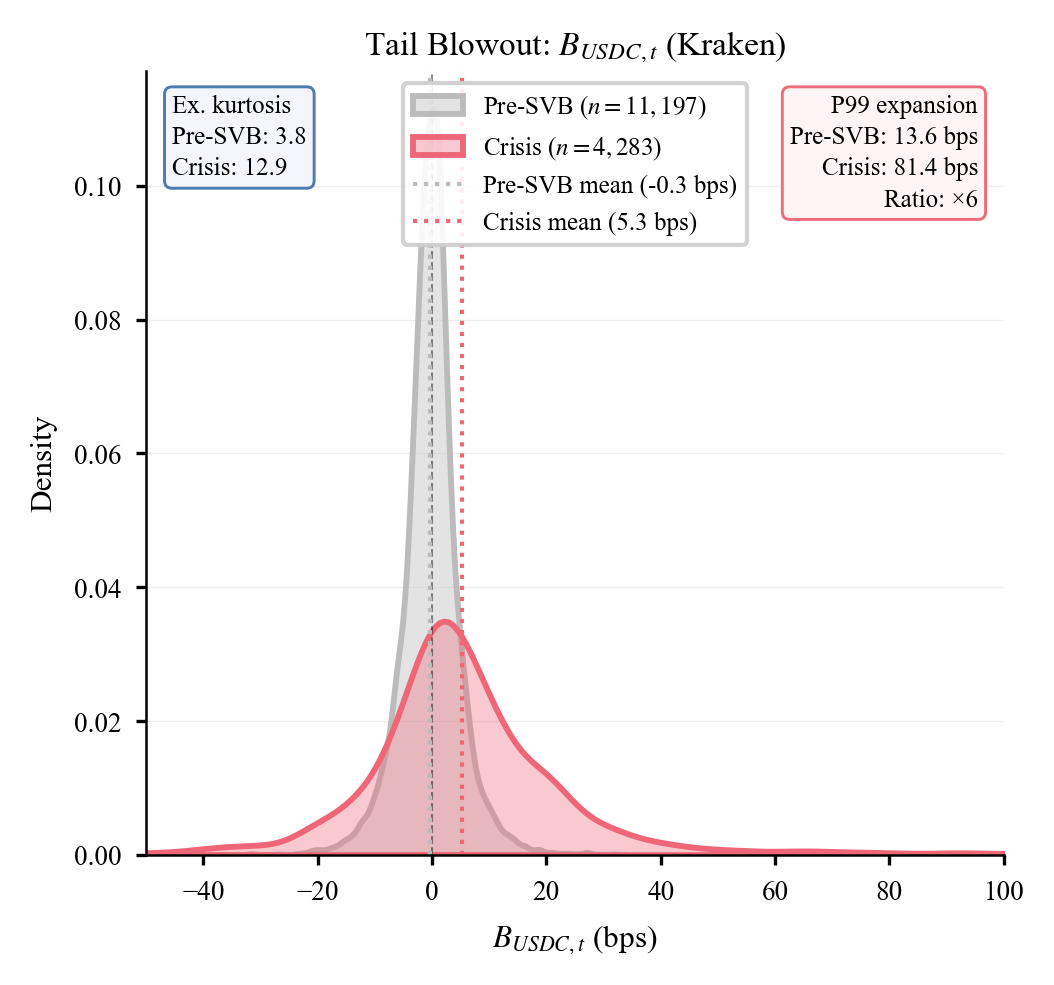
\includegraphics[width=\columnwidth]{figures_col/fig_tail_blowout_kde.png}
    \caption{Kraken distribution of USDC adjusted residual $B_{\text{USDC},t}$: pre-SVB vs.\ crisis. Crisis shows a right shift, excess kurtosis 12.9 (vs.\ 3.8), and a $6\times$ increase in the 99th percentile (13.6 to 81.4 bps).}
    \label{fig:tailblowout}
\end{figure}

% Single-column figure (portrait KDE -- fits in one column)

\paragraph{Distributional robustness.}
\begin{sloppypar}
Chow tests reject parameter stability at March~10 for $D_t$ ($F{=}2{,}089$), $B_t$ ($F{=}230$), and AR(1) dynamics ($F{=}71$; all $p{<}10^{-16}$), validating the regime split \cite{chow1960}. Table~\ref{tab:dist_robust} shows the USDC crisis $B_t$ has excess kurtosis 12.9 and skewness $+1.01$ (vs.\ pre-SVB 3.8/${\approx}$0), and the USDT crisis kurtosis is only 1.4, confirming USDC-specific tail risk. Jarque--Bera rejects normality throughout (USDC crisis JB${=}$30,498). Cross-stablecoin correlation drops from 0.44 to 0.16 in crisis, consistent with divergent dynamics rather than a common shock.
\end{sloppypar}

\begin{table}[H]
\label{tab:dist_robust}
\footnotesize
\resizebox{0.90\columnwidth}{!}{%
\begin{tabular}{llcccc}
\toprule
Channel & Regime  & Skewness & Ex.Kurt. & Min  & Max   \\
\midrule
USDC & Pre  &  0.00 &  3.8 & $-$36.9 &  32.0 \\
USDC & Crisis   &  1.01 & 12.9 & $-$165.2 & 180.6 \\
USDC & Post &  0.30 &  2.8 & $-$43.2 &  79.4 \\
USDT & Pre  & -0.36 &  5.2 & $-$36.4 &  34.5 \\
USDT & Crisis   & -0.11 &  1.4 & $-$26.8 &  29.9 \\
USDT & Post & -0.03 &  2.0 & $-$37.8 &  36.2 \\
\bottomrule
\end{tabular}
}
\caption{Higher-moment diagnostics for adjusted residual $B_t$ by regime. Excess kurtosis is Fisher ($0$ under Gaussian); Min/Max in bps.}
\end{table}

Figure~\ref{fig:corrheat} visualizes the decorrelation across all channels: pre-SVB cross-channel correlations ($B_{\text{USDC}}$--$B_{\text{USDT}}$: $0.44$) collapse in crisis ($0.16$) and partially recover post-SVB ($0.38$), while cross-exchange USDT channels remain tightly correlated throughout.

\begin{figure}[H]
    \centering
    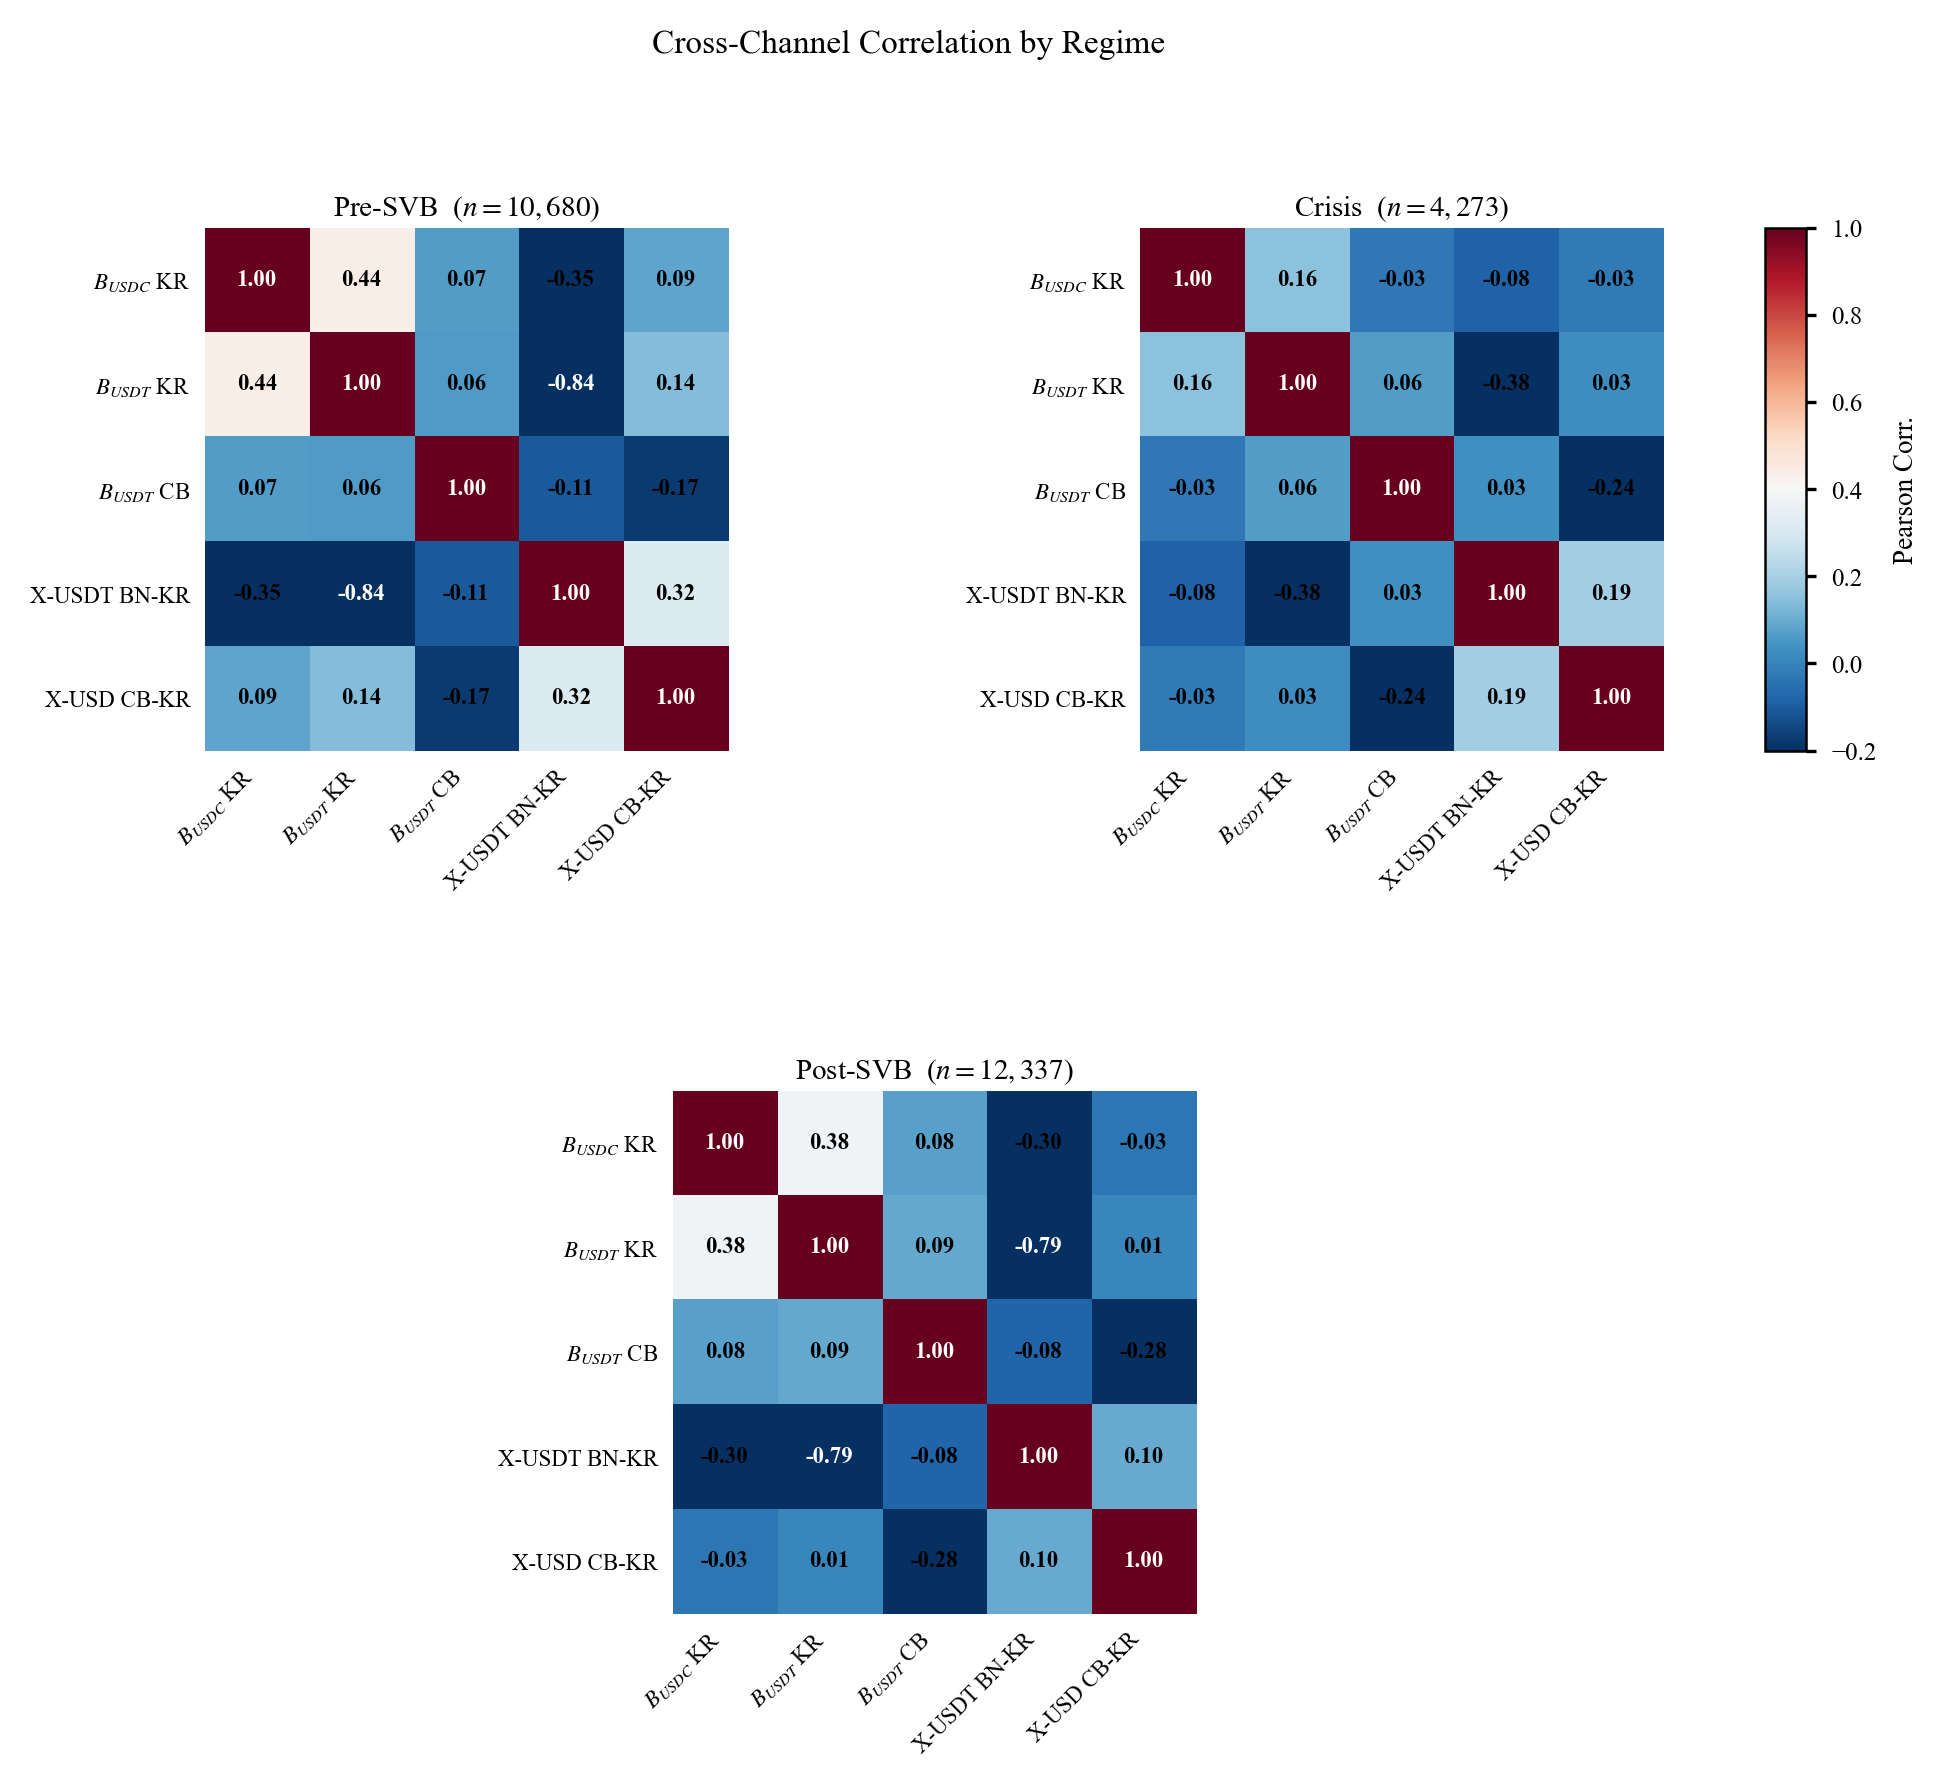
\includegraphics[width=\columnwidth]{figures_col/fig_correlation_regime_heatmap.png}
    \caption{Regime correlation heatmap for adjusted residuals and cross-exchange basis. $B_{\text{USDC}}$--$B_{\text{USDT}}$ correlation drops from $0.44$ to $0.16$ in crisis, indicating divergent stablecoin dynamics.}
    \label{fig:corrheat}
\end{figure}

\subsection{Price discovery}
Given the liquidity asymmetry documented above, as Coinbase BTC/USD is $26\times$ deeper than Kraken BTC/USDC, we want to know where price discovery occurs across these fragmented channels.

\begin{table}[H]
\label{tab:coint_vecm}
\footnotesize
\centering
\resizebox{\columnwidth}{!}{%
\begin{tabular}{lccccccl}
\toprule
Channel & Rank & $k_\Delta$ & Trace$_{r=0}$ & $\alpha_{\text{USD}}$ & $\alpha_{\text{other}}$ & IS$_{\text{USD}}$ [0.69,\,0.77] & Leader \\
\midrule
BTC/USD vs BTC/USDC & 0 & 2 &  7.71 & ---    & ---    & ---  & undetermined \\
BTC/USD vs BTC/USDT & 1 & 8 & 27.03 & 0.0079 & 0.0118 & 0.73 & BTC/USD \\
\bottomrule
\multicolumn{8}{l}{\footnotesize 95\% critical value for trace $r{=}0$: 15.49. IS = Hasbrouck (1995) midpoint; bounds [0.69,\,0.77].}
\end{tabular}%
}
\caption{Johansen cointegration and VECM price-discovery results for primary Kraken channels (no-FF sample).}
\end{table}

To determine the true informational anchor during crisis, we test for cointegration across Kraken's parallel quote currencies. Table~\ref{tab:coint_vecm} confirms BTC/USD and BTC/USDT share a stochastic trend (rank $=1$, stable at $k_\Delta\pm1$). To quantify this leadership, we compute Hasbrouck (1995) Information Share bounds \cite{hasbrouck1995}. Across both Cholesky orderings, we isolate an $\text{IS}_{\text{USD}}\in[0.69,\,0.77]$ (midpoint $\mathbf{0.73}$), proving fiat BTC/USD drives ${\approx}73\%$ of permanent price discovery. This tight width ($0.08$) and high residual correlation ($0.889$) confirm strong, ordering-independent structural leadership. Conversely, the highly distressed BTC/USDC pair fails to reject rank $=0$ under strict no-forward-fill sampling, reflecting profound quote instability during this short window.

Complementing these structural findings, Figure~\ref{fig:irf} maps high-frequency shock transmission via orthogonalized impulse-response functions (IRFs). Derived from a bivariate VAR on 1-minute returns (AIC-selected 10 lags, ordering BTC/USD first, $N{=}26{,}548$), the results reveal a stark asymmetry. A fiat BTC/USD shock transmits instantly to BTC/USDC (Panel~C: ${\approx}6$ bps impact, decaying over 3--4 minutes). In sharp contrast, the reverse transmission (Panel~B) is statistically indistinguishable from zero, with the 95\% confidence interval enveloping zero at all horizons. This definitive asymmetry confirms that deep fiat markets dictate price discovery, forcing fragmented stablecoin pairs to adjust.

\begin{figure}[H]
    \centering
    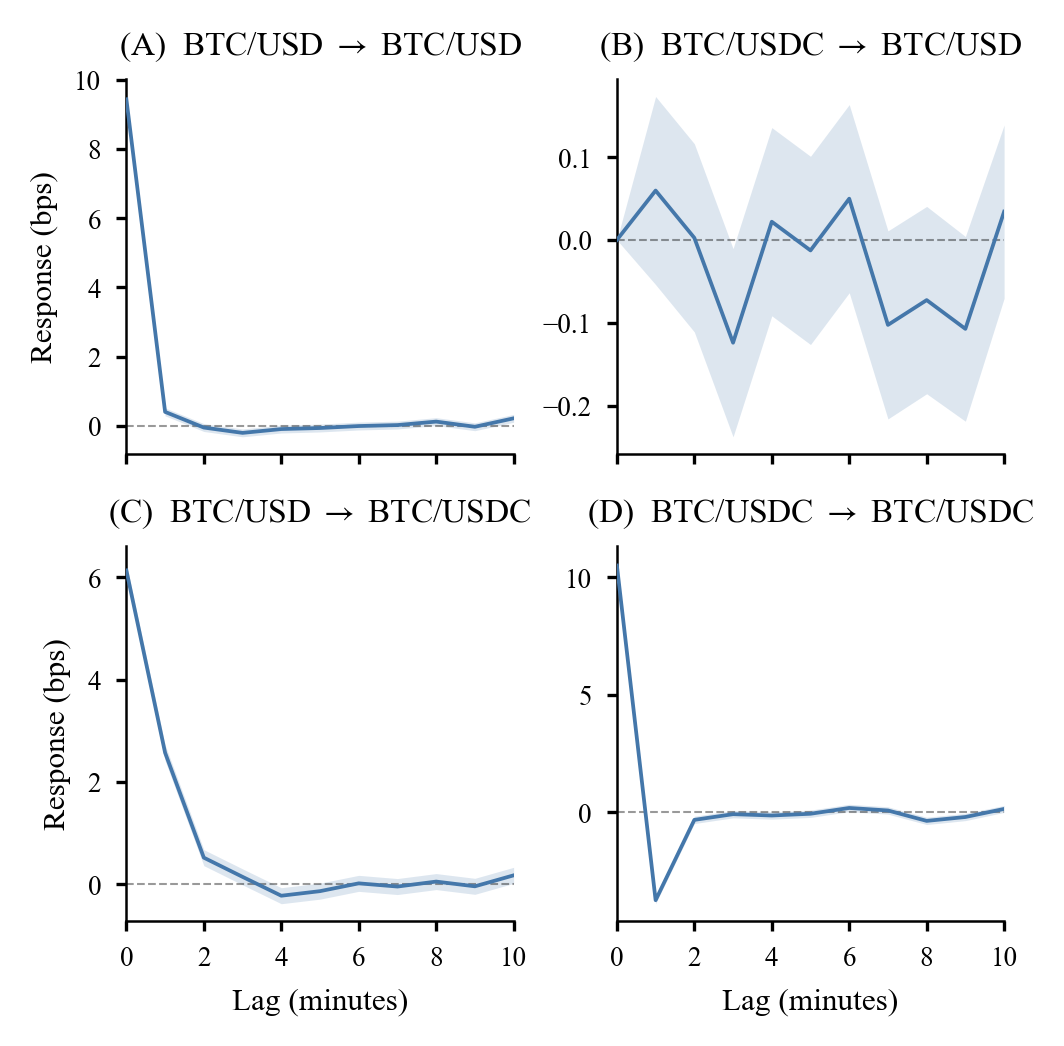
\includegraphics[width=\columnwidth]{figures_col/fig_var_irf.png}
    \label{fig:irf}
    \caption{Orthogonalized IRF from VAR(10) on Kraken BTC/USD and BTC/USDC returns (bps). (B)~USDC$\to$USD: insignificant. (C)~USD$\to$USDC: significant (${\approx}6$ bps, decays in 3--4 min). Shaded: 95\% asymptotic CI.}
\end{figure}

BH/FDR-corrected Granger tests on returns provide secondary evidence: BTC/USD $\to$ BTC/USDC is significant ($q<0.001$) but the reverse is not after FDR correction ($q=0.13$), consistent with fiat-to-stablecoin price adjustment. All other channels (USDT intra-exchange, cross-exchange) show bidirectional significance, consistent with active two-way arbitrage in more liquid markets.

\subsection{Arbitrage after fees}\label{sec:arb}
Having established that price discovery resides in the fiat-quoted channel, a natural question is whether the documented dislocations offer exploitable arbitrage opportunities. We evaluate this using explicit trade construction---3-leg triangular for intra-exchange stablecoin channels, 2-leg pre-funded buy/sell for cross-exchange---under two cost bounds:
\begin{align}
    \text{cost}^{\text{fee}}_t &= n_{\text{legs}}\cdot f, \\
    \text{cost}^{\text{fee+slip}}_t &= n_{\text{legs}}\cdot f + \sum_{\ell=1}^{n_{\text{legs}}}\tfrac{1}{2}\,\text{RangeProxy}_{\ell,t},
\end{align}
with $f=5$ bps per taker leg.

% Full-width figure (two panels)
\begin{figure}[H]
    \centering
    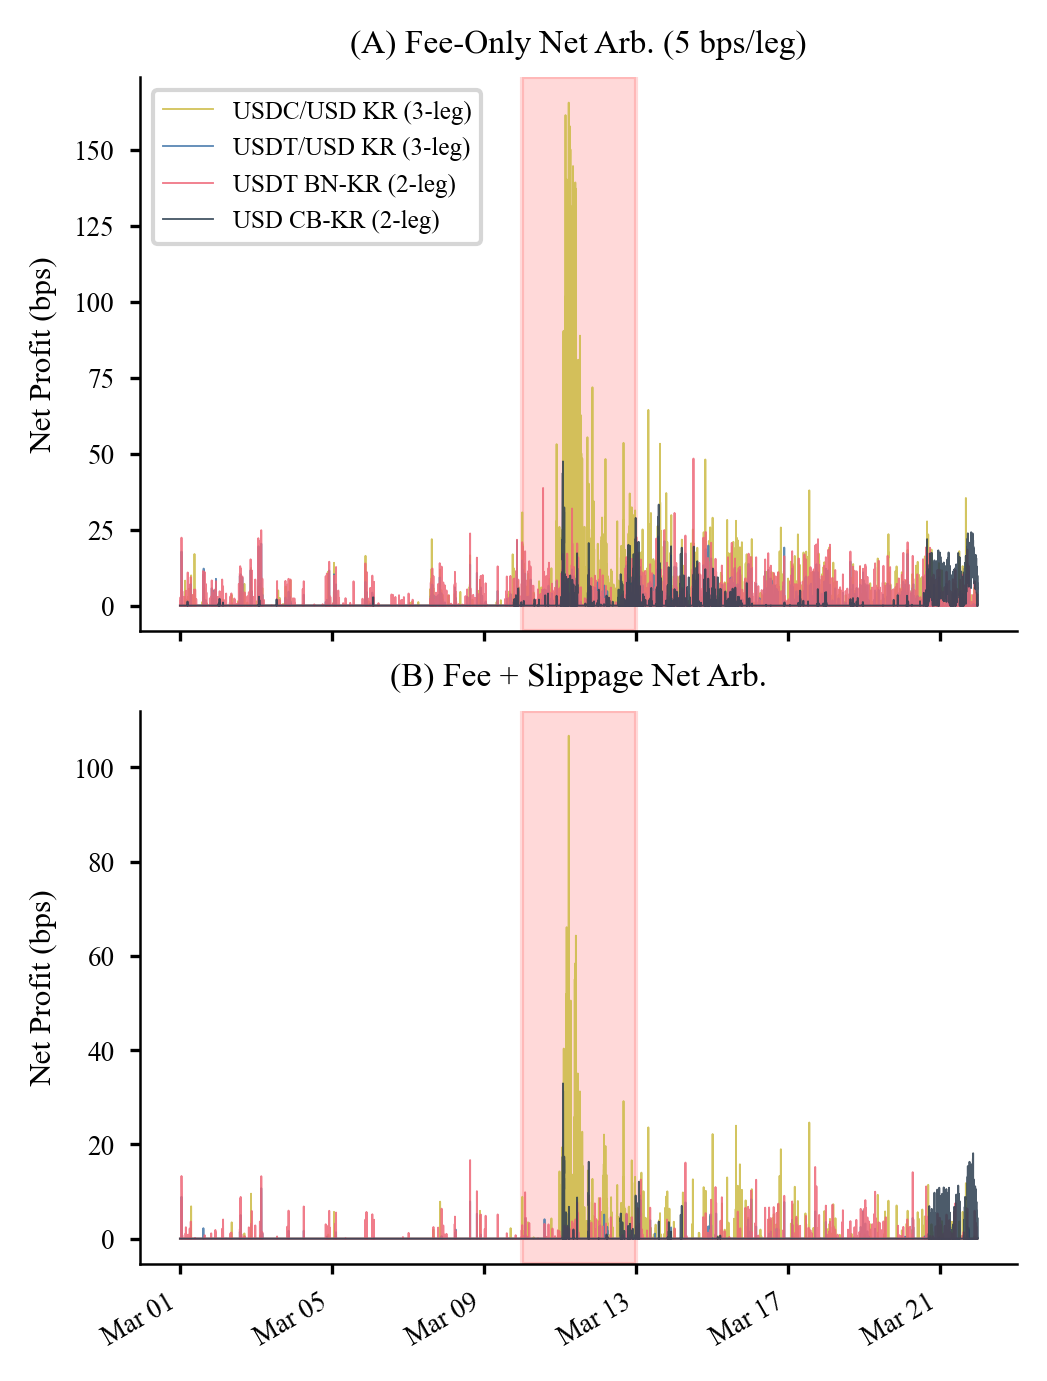
\includegraphics[width=\columnwidth]{figures_col/fig_arbitrage_after_fees.png}
    \caption{Net arbitrage profit (bps) under (A) fee-only costs (5 bps/leg) and (B) fee + range-based slippage. Crisis USDC profits compress sharply with slippage; cross-exchange profits are also attenuated.}
    \label{fig:arbfees}
\end{figure}

Figure~\ref{fig:arbfees} shows the time series of net arbitrage profits under both cost specifications. Adding range-based slippage (Panel~B) materially compresses profitability: USDC intra-exchange crisis profitability falls from $29.16\%$ to $6.72\%$ (net $4.83$ to $0.64$ bps); Coinbase--Kraken BTC/USD falls from $11.32\%$ to $2.29\%$. Fee sensitivity: at $f{=}3$ bps (maker rebate), USDC crisis fee+slippage profitability rises to $14.0\%$; at $f{=}10$ bps (retail), it falls to $1.0\%$. The narrow post-cost opportunities are consistent with limited executable arbitrage under realistic frictions.

\begin{table}[H]
\label{tab:arb}
\footnotesize
\resizebox{\columnwidth}{!}{%
\begin{tabular}{llcrr}
\toprule
Channel & Regime & Cost Variant & \%Profitable & AvgNetUncond (bps) \\
\midrule
USDC/USD (Kraken)      & Crisis   & Fee-only & 29.16 & 4.83 \\
USDC/USD (Kraken)      & Crisis   & Fee+slip &  6.72 & 0.64 \\
USDC/USD (Kraken)      & Post-SVB & Fee-only &  9.38 & 0.56 \\
USDC/USD (Kraken)      & Post-SVB & Fee+slip &  1.78 & 0.08 \\
USDT/USD (Kraken)      & Crisis   & Fee-only &  3.76 & 0.14 \\
USDT/USD (Kraken)      & Crisis   & Fee+slip &  0.37 & 0.01 \\
Cross BTC/USD (CB--KR) & Crisis   & Fee-only & 11.32 & 0.72 \\
Cross BTC/USD (CB--KR) & Crisis   & Fee+slip &  2.29 & 0.15 \\
Cross BTC/USDT (BN--KR)& Crisis   & Fee-only & 11.85 & 0.49 \\
Cross BTC/USDT (BN--KR)& Crisis   & Fee+slip &  1.81 & 0.05 \\
\bottomrule
\end{tabular}%
}
\caption{Arbitrage profitability by channel/regime with 5 bps taker fees per leg (3-leg intra-exchange; 2-leg cross-exchange).}
\end{table}

\section{Regulatory Interpretation}\label{sec:regulation}
% ======================================================================



Our analysis identifies a definitive failure chain: banking-layer reserve-access risk drives fiat peg deviation, which subsequently drives crypto-market dispersion. This transmission occurs exogenously (mechanical shock $D_t$) and endogenously via the microstructural contagion channel ($\hat\lambda$). With liquidity constraints imposing a structural ceiling on arbitrage efficiency, Circle's localized \$3.3B SVB exposure \cite{circle2023} serves as the root of this breakdown. The ${\sim}940\times$ half-life gap (bootstrap $p{<}10^{-4}$) localizes the persistent dislocation to the peg layer, while $\hat\lambda$ confirms active market propagation. Because sustained recovery required emergency federal deposit guarantees \cite{jointstatement2023}, we evaluate whether the GENIUS Act adequately targets this exact failure chain.

\begin{table}[H]
\label{tab:genius_cf}
\footnotesize
\resizebox{\columnwidth}{!}{%
\begin{tabular}{p{3.5cm}rrrp{4.8cm}}
\toprule
Scenario & Mitigation (\%) & Implied $D_t$ (bps) & Reduction (bps) & Policy mapping \\
\midrule
Observed baseline        &   0 & 320.0 &   0.0 & SVB/No GENIUS baseline \\
Low mitigation           &  25 & 240.0 &  80.0 & Reserve composition + redemption + transparency \\
Moderate mitigation      &  50 & 160.0 & 159.9 & Reserve composition + redemption + transparency \\
High mitigation          &  75 &  80.1 & 239.9 & Reserve composition + redemption + transparency \\
Full-mitigation lower bd & 100 &   0.1 & 319.9 & Reserve composition + redemption + transparency \\
\bottomrule
\end{tabular}%
}
\caption{Illustrative GENIUS Act scenario range (not causal): assumed mitigation of the reserve lock-up shock mapped to implied crisis $D_t$ means from observed moments.}
\end{table}

The GENIUS Act (July 2025) targets four dimensions of this transmission mechanism \cite{genius2025}. We map our empirical results directly to these provisions: (i)~\textit{Reserve composition}: Table~\ref{tab:genius_cf} implies a 25\%--75\% mitigation compresses $D_t$ to ${\approx}240$--$80$ bps. (ii)~\textit{Timely redemption}: The $572$-minute peg half-life quantifies the market impact of a five-day redemption freeze. (iii)~\textit{Bankruptcy super-priority}: This mandate addresses extreme P99 tail risk expansion ($81.4$ vs.\ $13.6$ bps). (iv)~\textit{Transparency}: Circle's delayed disclosure drove the violent USDC--USDT decorrelation ($\rho{=}0.16$). Ultimately, the persistent $+2.18$ bps cross-exchange premium and $26\times$ depth gap suggest reserve-layer reforms cannot entirely eliminate spatial fragmentation.

% ======================================================================
\section{Conclusion}\label{sec:conclusion}
% ======================================================================

Our framework yields four integrated findings. First, SVB-triggered fragmentation is strictly attributable to stablecoin peg risk: while $D_t$ reaches $+320$ bps, $B_t$ remains compressed near $+5$ bps with sub-minute mean reversion. The statistically confirmed ${\sim}940\times$ half-life gap ($p{<}10^{-4}$) localizes persistent dislocation entirely to reserve-access risk. Second, fiat stress actively infects the adjusted basis beyond mechanical repricing; the transmission parameter $\hat\lambda$ becomes highly significant during crisis ($p{<}0.001$), with USDC and USDT propagating stress oppositely. Third, this USDC-specific shock is evidenced by extreme tail expansion (excess kurtosis $12.9$), a persistent USDT safe-haven premium ($+58$ bps), and violent cross-stablecoin decorrelation ($0.44\to0.16$). Fourth, executable post-friction arbitrage narrows sharply ($29\%\to7\%$), heavily constrained by a $26\times$ depth gap.

The GENIUS Act targets this exact failure chain. Because dislocation originates in the peg layer and propagates via the $\lambda$ contagion channel, mitigating reserve-access risk should mechanically compress $D_t$ while simultaneously dampening $B_t$. However, persistent cross-exchange deviations suggest additional market-structure measures may still be required. A post-GENIUS replication study during a future systemic stress event is a natural extension.

\paragraph{Interpretation boundaries.} This evidence remains observational and window-specific (March 2023). Thus, $\hat\lambda$ captures Granger-predictive transmission rather than structural causation, and our policy mappings serve as consistency checks rather than causal identification. Nevertheless, the empirical foundation is highly robust: (i)~HAC standard errors preserve all directional signs; (ii)~no-forward-fill filters maintain rank-order conclusions; (iii)~$\hat\lambda$ contagion survives both no-FF and 5-minute sampling; (iv)~cointegration remains rank-stable for BTC/USD--USDT but correctly breaks down for the distressed USDC channel; and (v)~Chow tests definitively validate the regime split.

\newpage

\small
\begin{thebibliography}{99}
\bibitem{amihud2002} Amihud, Y. (2002). Illiquidity and stock returns: Cross-section and time-series effects. {Journal of Financial Markets}, 5(1), 31--56.
\bibitem{chow1960} Chow, G. C. (1960). Tests of equality between sets of coefficients in two linear regressions. {Econometrica}, 28(3), 591--605.
\bibitem{circle2023} Circle (March 11, 2023). {Silicon Valley Bank and USDC}. Circle update.
\bibitem{englegranger1987} Engle, R. F., \& Granger, C. W. J. (1987). Co-integration and error correction: Representation, estimation, and testing. {Econometrica}, 55(2), 251--276.
\bibitem{jointstatement2023} Federal Reserve, FDIC, and U.S. Treasury (March 12, 2023). {Joint statement by the Department of the Treasury, Federal Reserve, and FDIC}.
\bibitem{granger1969} Granger, C. W. J. (1969). Investigating causal relations by econometric models and cross-spectral methods. {Econometrica}, 37(3), 424--438.
\bibitem{hasbrouck1995} Hasbrouck, J. (1995). One security, many markets: Determining the contributions to price discovery. {Journal of Finance}, 50(4), 1175--1199.
\bibitem{johansen1988} Johansen, S. (1988). Statistical analysis of cointegration vectors. {Journal of Economic Dynamics and Control}, 12(2--3), 231--254.
\bibitem{neweywest1987} Newey, W. K., \& West, K. D. (1987). A simple, positive semi-definite, heteroskedasticity and autocorrelation consistent covariance matrix. {Econometrica}, 55(3), 703--708.
\bibitem{roll1984} Roll, R. (1984). A simple implicit measure of the effective bid-ask spread in an efficient market. {Journal of Finance}, 39(4), 1127--1139.
\bibitem{genius2025} U.S. Congress (2025). {Public Law 119-27: Guiding and Establishing National Innovation for U.S. Stablecoins Act (GENIUS Act)}.
\end{thebibliography}

\end{document}]
